\documentclass[../Text/00main.tex]{subfiles}
\graphicspath{{../}}

\begin{document}



\chapter{Additional figures from methods}

\section{Table of CSCS Piz daint specifications}\label{app:pizdaint}

\begin{figure}[htb!]
    \centering
    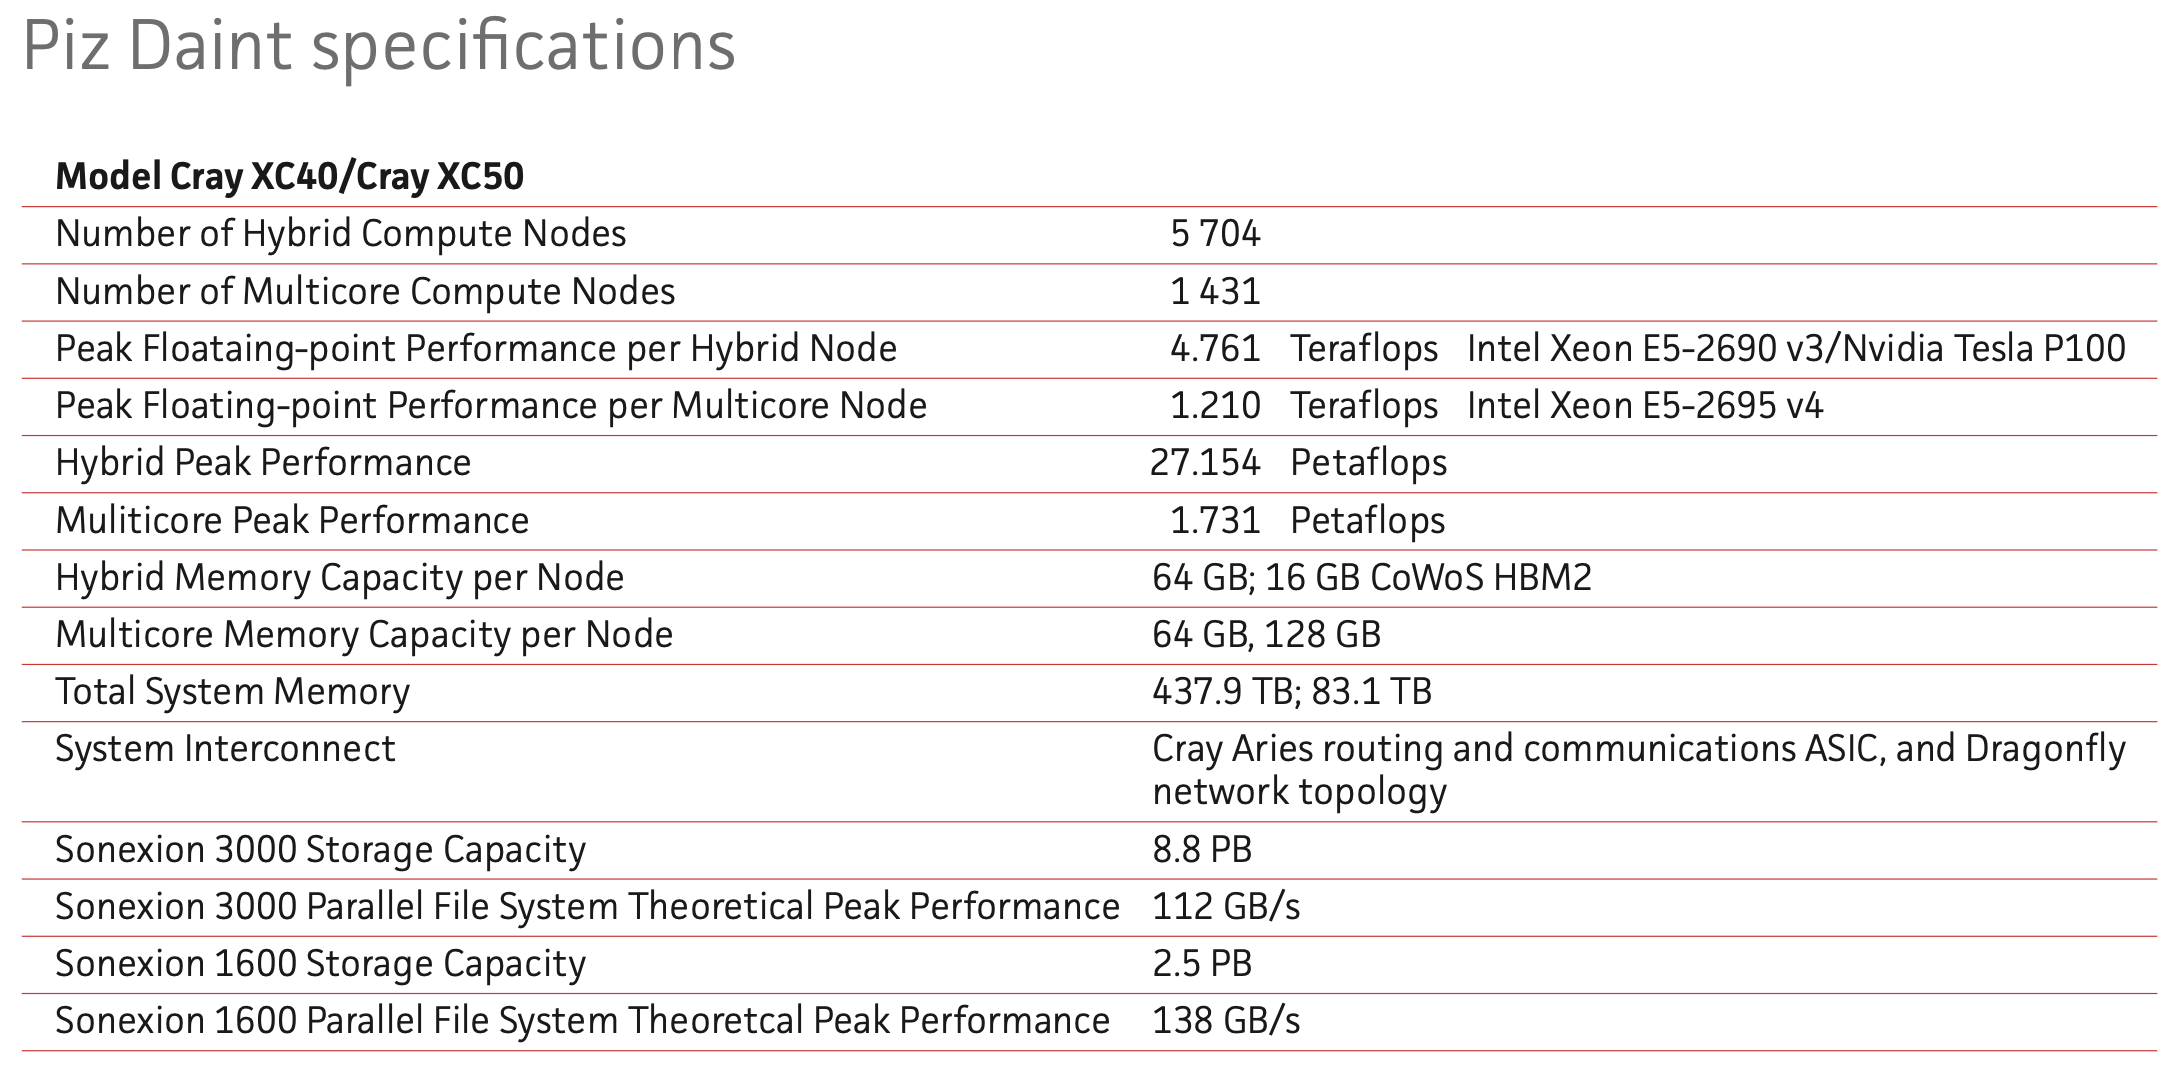
\includegraphics[width=.98\linewidth]{images_methods/Pizdainttable.png}
    \caption{Table of specifications of the Piz Daint HPC. }
    \label{fig:my_label}
\end{figure}
\FloatBarrier
\section{More elaborate workflow description}\label{app:software}

\section{Moment tensor starting composition}\label{app:sdrvar_methods}

\begin{figure}[htb!]
    \centering
    
    \subfloat[CMT1]{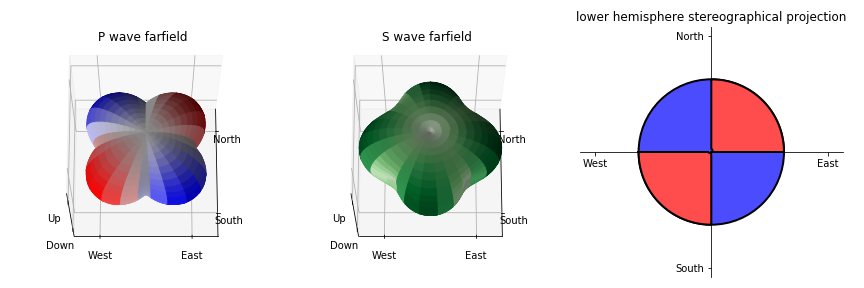
\includegraphics[width=15cm]{images_results/rp1.png}}%
  
    \subfloat[CMT2]{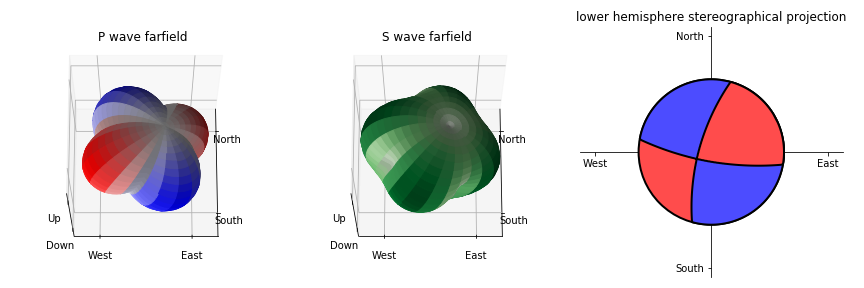
\includegraphics[width=15cm]{images_results/rp2.png}}%

    \subfloat[CMT3]{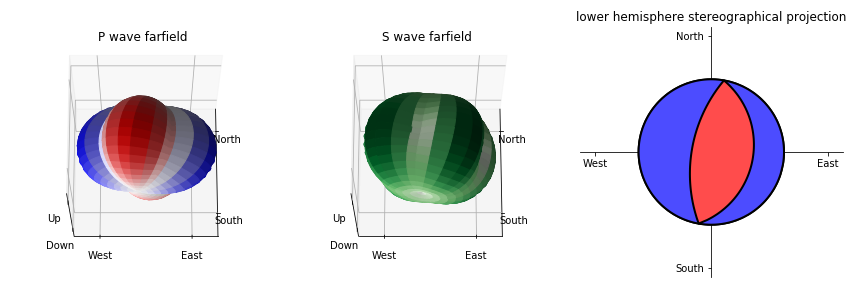
\includegraphics[width=15cm]{images_results/rp3.png}}%

    \subfloat[CMT4]{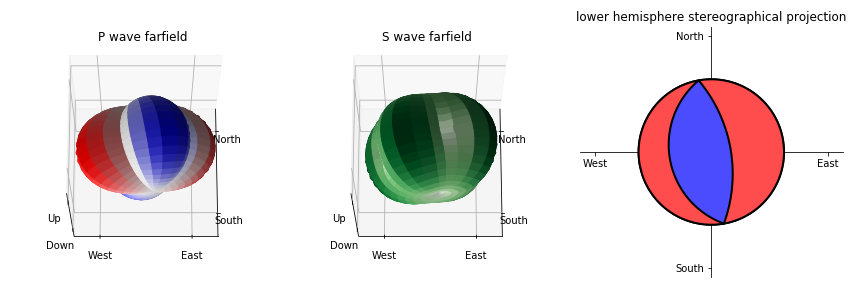
\includegraphics[width=15cm]{images_results/rp4.png}}%
     
    
    \caption{Starting configurations of CMT1-4 with the P wave field, S wave field and the focal mechanism Obtained by Obspy \citep{hosseini_obspydmt_2017}, \citep{krischer2015obspy}.}%
    \label{fig:starting_patterns}%
\end{figure}


\FloatBarrier
\begin{figure}[htb!]
    \centering
    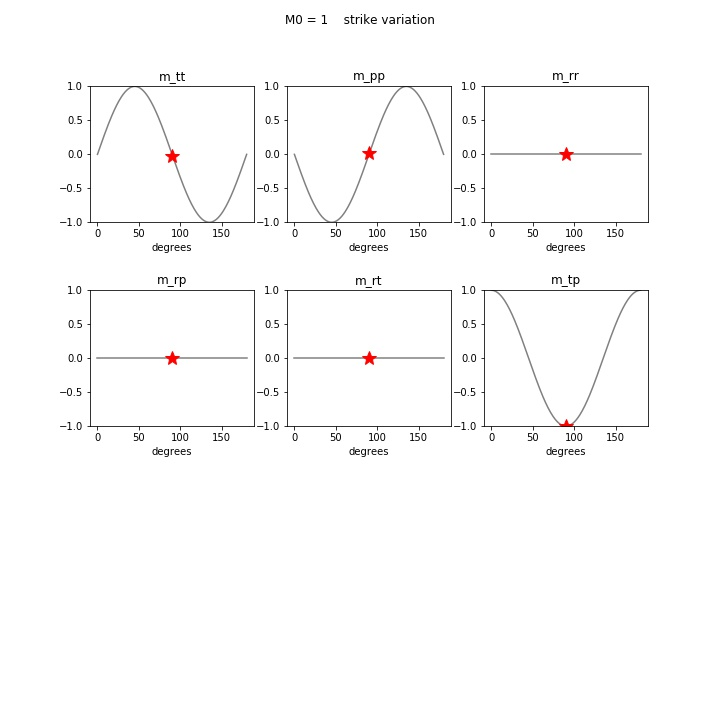
\includegraphics[width=1.0\textwidth, trim= 0cm 10cm 0cm 0cm,clip]{images_methods/strikevar.jpg}
    \caption{CMT components for strike variation with CMT1 as starting configuration at dip 90 and rake 180$\degree$.}
    \label{figapp: strikevar}
\end{figure}

\begin{figure}[htb!]
    \centering
    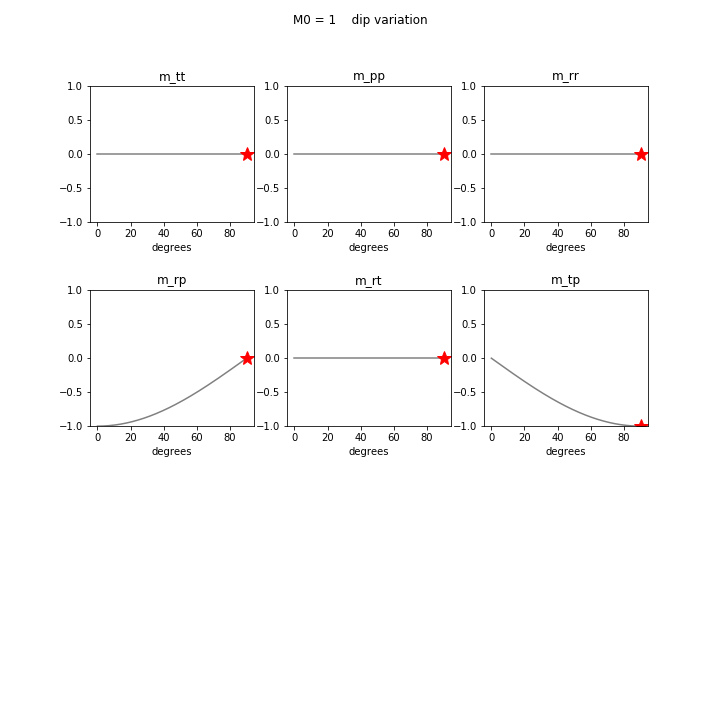
\includegraphics[width=1.0\textwidth, trim= 0cm 10cm 0cm 0cm,clip]{images_methods/dipvar.png}
    \caption{CMT components for dip variation with CMT1 as starting configuration at strike 90$\degree$ and rake 180$\degree$}
    \label{figapp: dipvar}
\end{figure}

\begin{figure}[htb!]
    \centering
    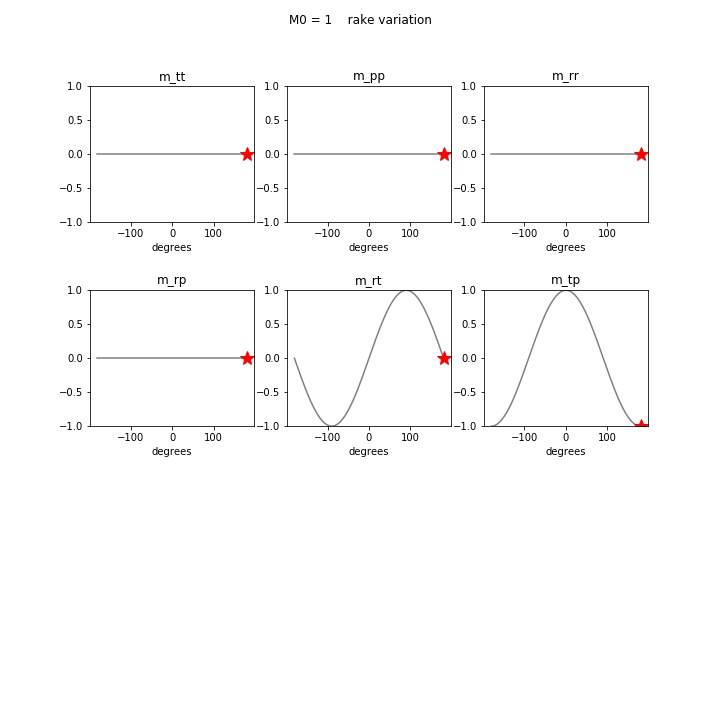
\includegraphics[width=1.0\textwidth, trim= 0cm 10cm 0cm 0cm,clip]{images_methods/rakevar.jpg}
    \caption{CMT components for rake variation with CMT1 as starting configuration at strike 90$\degree$ and dip 90$\degree$}
    \label{figapp: rakevar}
\end{figure}

\FloatBarrier

\chapter{Additional result figures}

\section{More images of waveforms from the validation}\label{app:validation}

\section{PGA vs PGV pattern}\label{app:PGAsame}

\begin{figure}
    \centering
    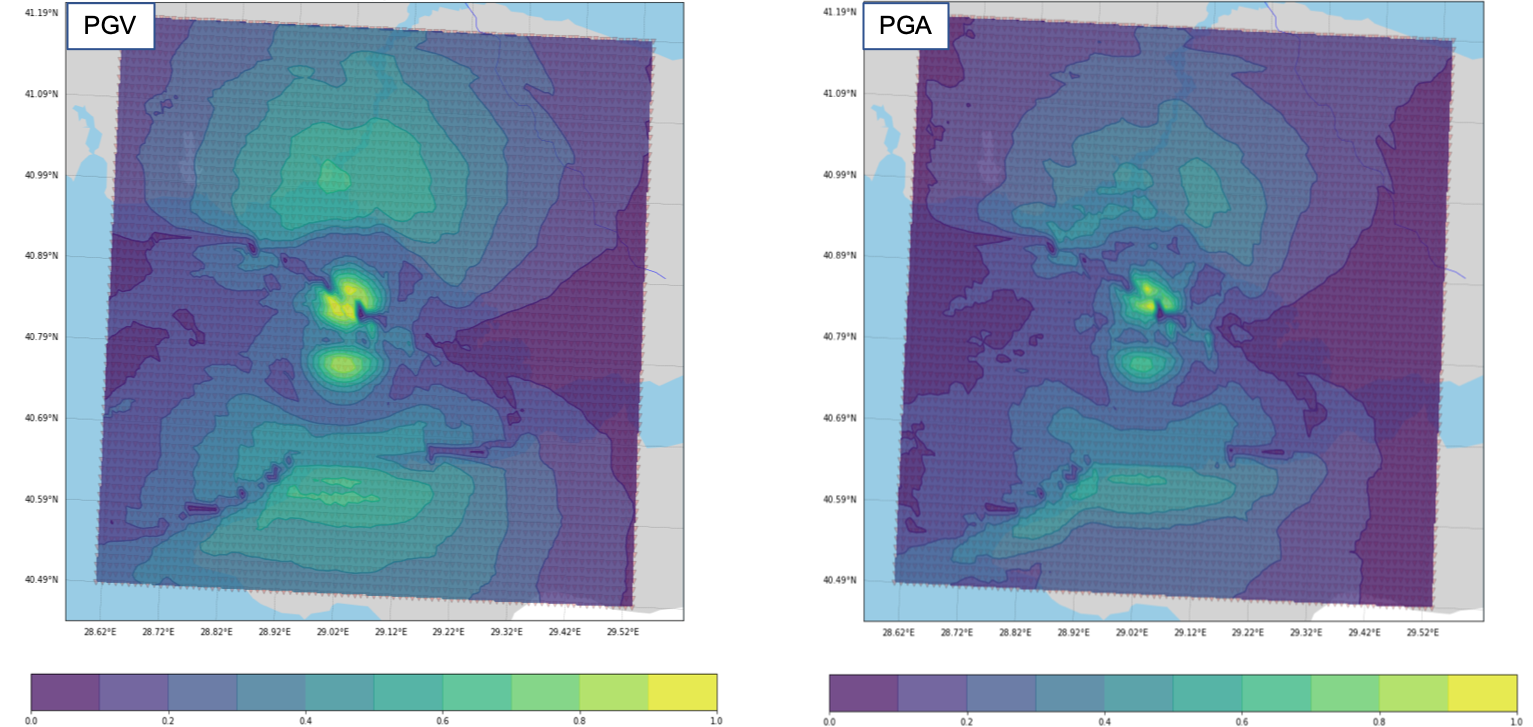
\includegraphics[width=\textwidth]{images_results/PGAVSPGV.png}
    \caption{PGV pattern compared with PGA pattern for CMT1 with model 3D + topo + ocean.}
    \label{figapp:pgapgvcompare}
\end{figure}

\FloatBarrier

\section{Additional images of different start configurations}{\label{app:morereffigs}}

\subsection{Reference scenarios CMT3 and CMT4}

\subsubsection{CMT3}

\begin{figure}[h]
    \centering
    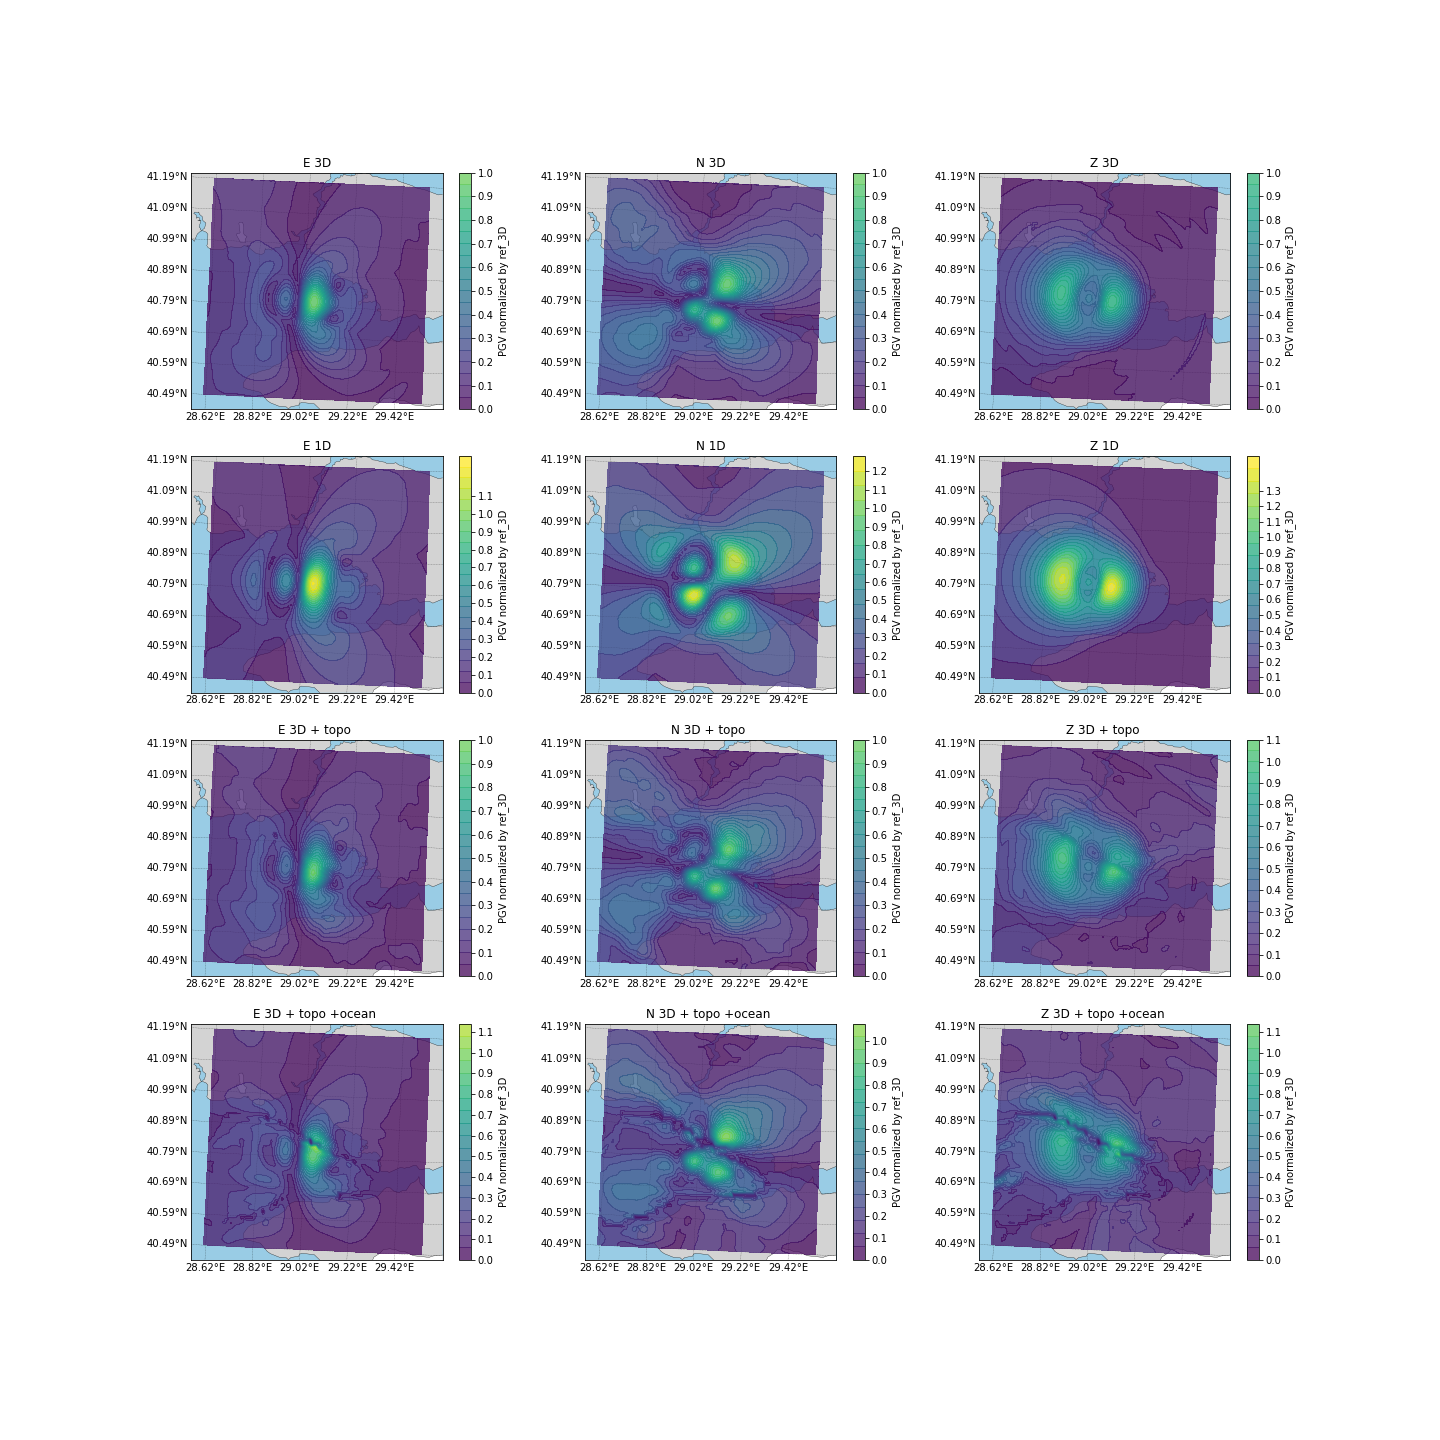
\includegraphics[width=1\linewidth]{images_results/Ref_scenarios_normalized_sc3.png}
    \caption{PGV reference scenario CMT3, strike 10, dip 30, rake 90, normalized with respect to the 3D configuration (top row).}
    \label{fig:ref_CMT3}
\end{figure}

\FloatBarrier

\subsubsection{CMT4}

\begin{figure}[h]
    \centering
    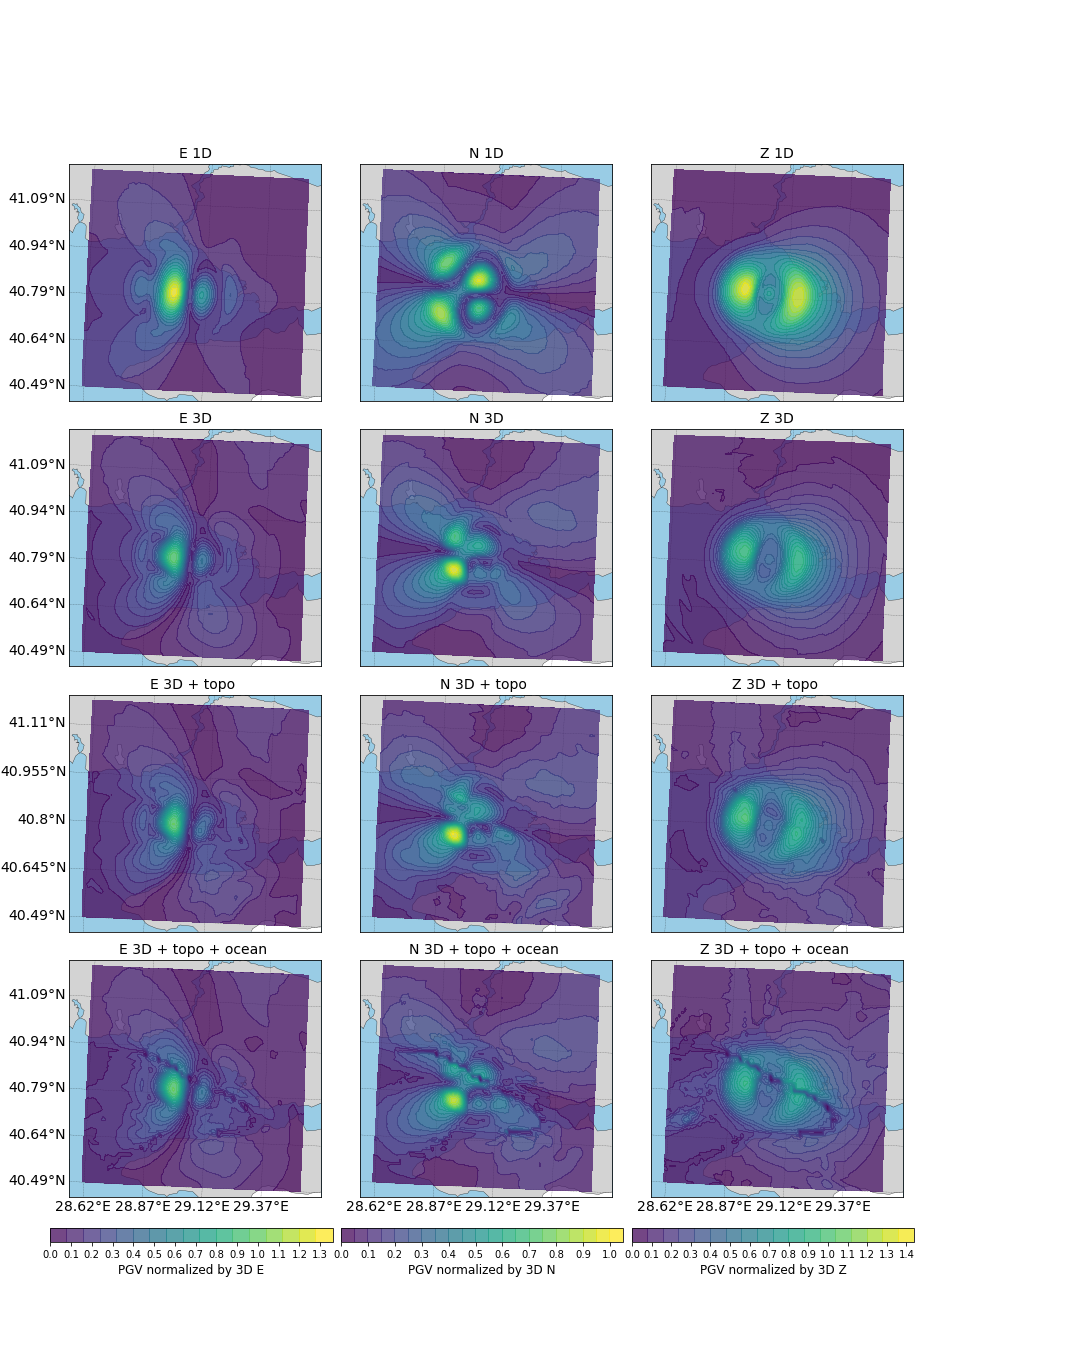
\includegraphics[width=1\linewidth]{images_results/Ref_scenarios_normalized_sc4.png}
    \caption{PGV reference scenario CMT4, strike -10, dip 60, rake -90, normalized with respect to the 3D configuration (top row).}
    \label{fig:ref_CMT4}
\end{figure}

\FloatBarrier

\subsection{Variation strike figures CMT3 and CMT4}

\subsubsection{CMT2}

\begin{figure}
    \centering
    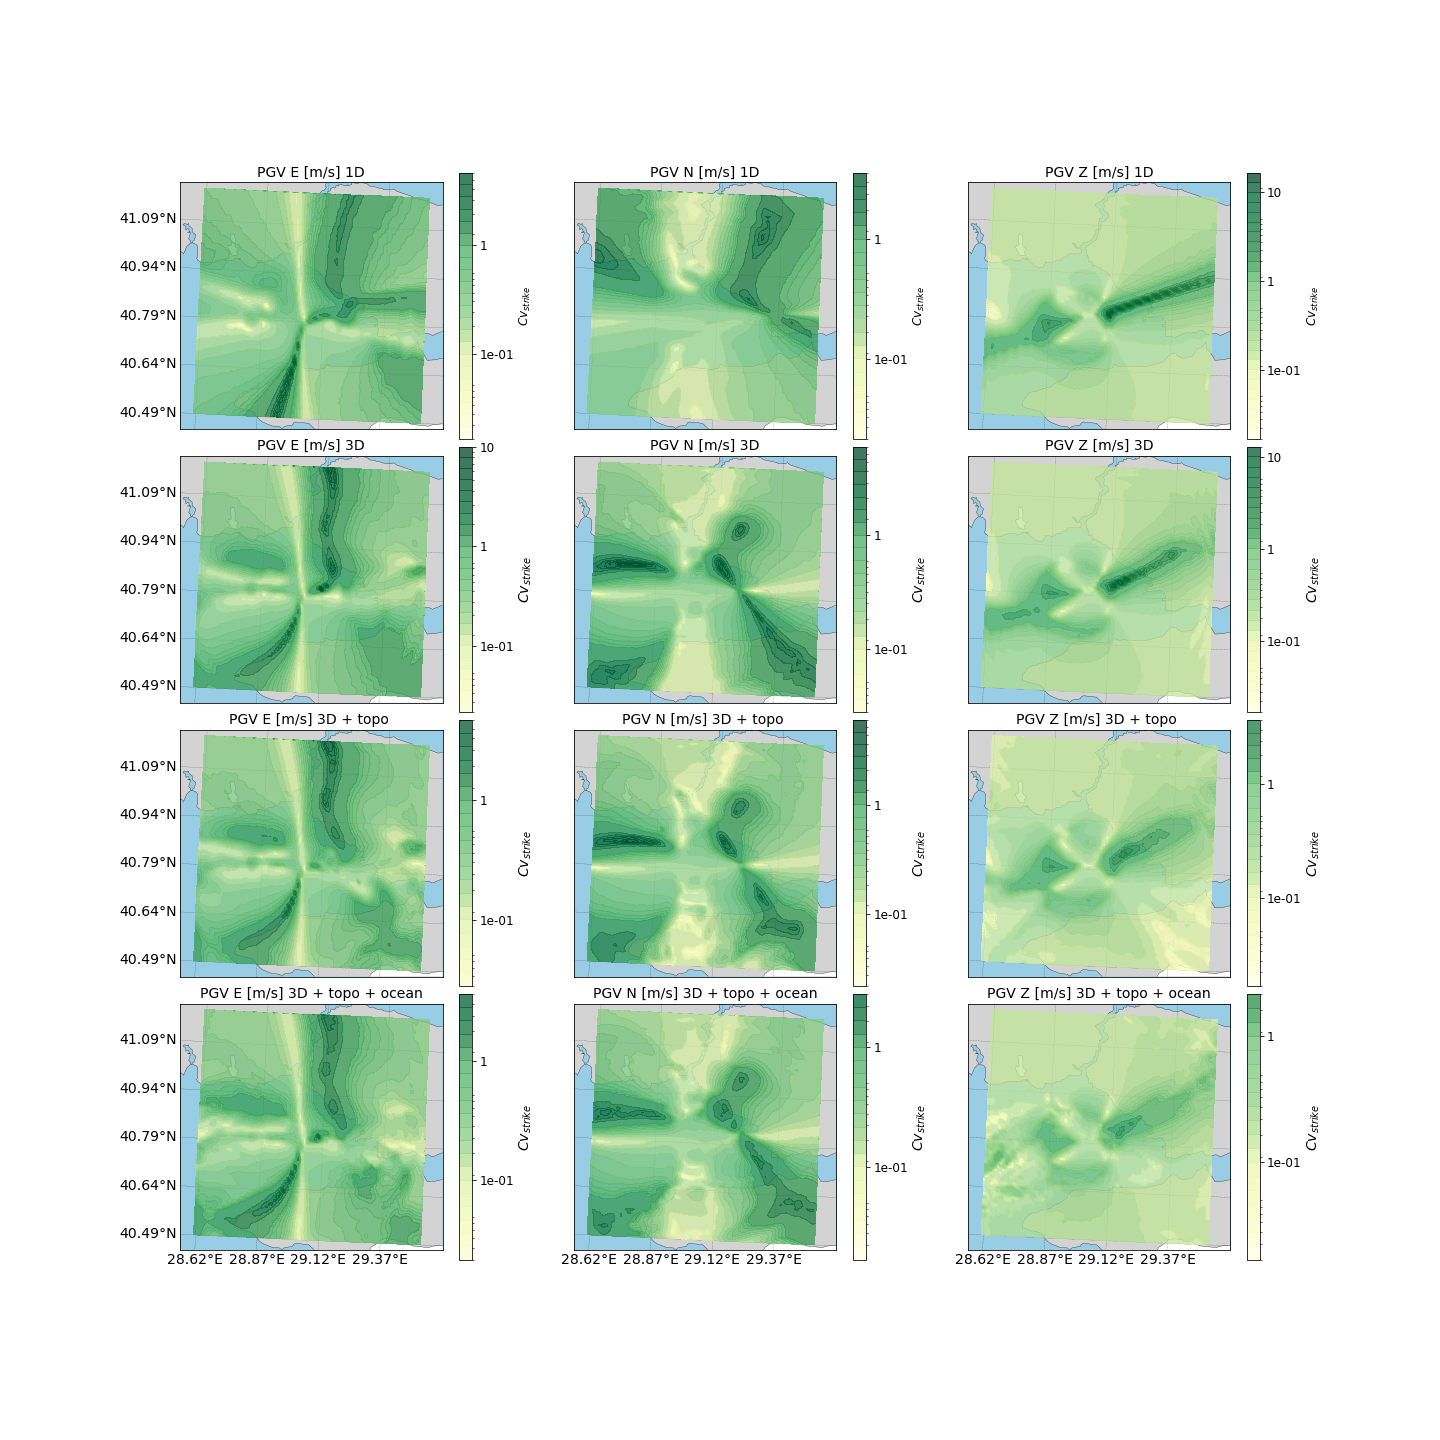
\includegraphics[width=1\linewidth,trim = 2cm 5cm 1cm 5cm, clip]{images_results/strike_variation_sigma_sc2.png}
    \caption{CMT2 coefficient of variation $Cv$ of strike variation, for each model domain in E, N and Z direction. Colourbar set to logarithmic to adequately show the large differences.}
    \label{fig:cmt2sigm}
\end{figure}


\begin{figure}[!h]
    \centering
    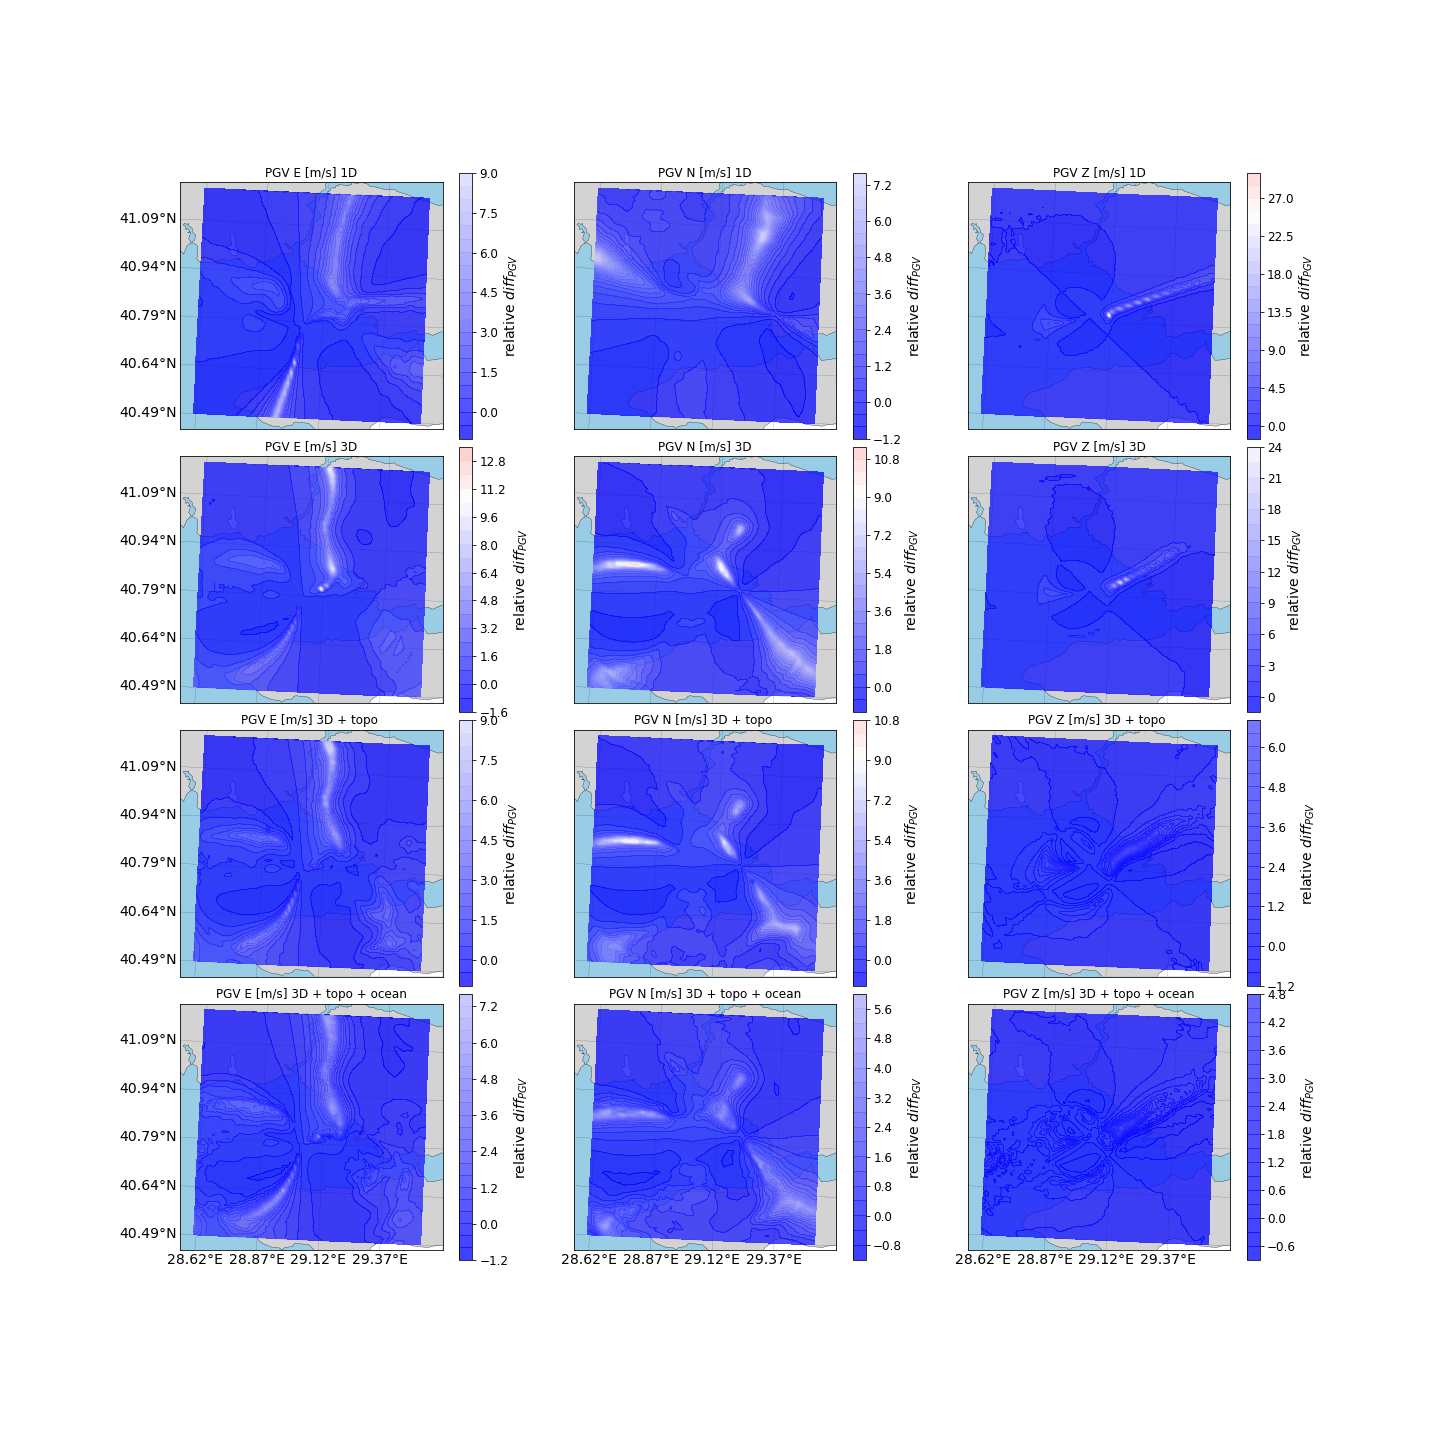
\includegraphics[width=1\linewidth,trim = 2cm 5cm 1cm 5cm, clip]{images_results/strike_variation_epsilon12_sc2.png}
    \caption{CMT2 relative difference between a scenario with a strike variation of 11.25$\degree$ with respect to the reference scenario. Colourbar set to the total minima and maxima of the 11.25$\degree$ and 22.5$\degree$ plots for comparison.}
    \label{fig:ref_eps12-2}
\end{figure}

\begin{figure}[!h]
    \centering
    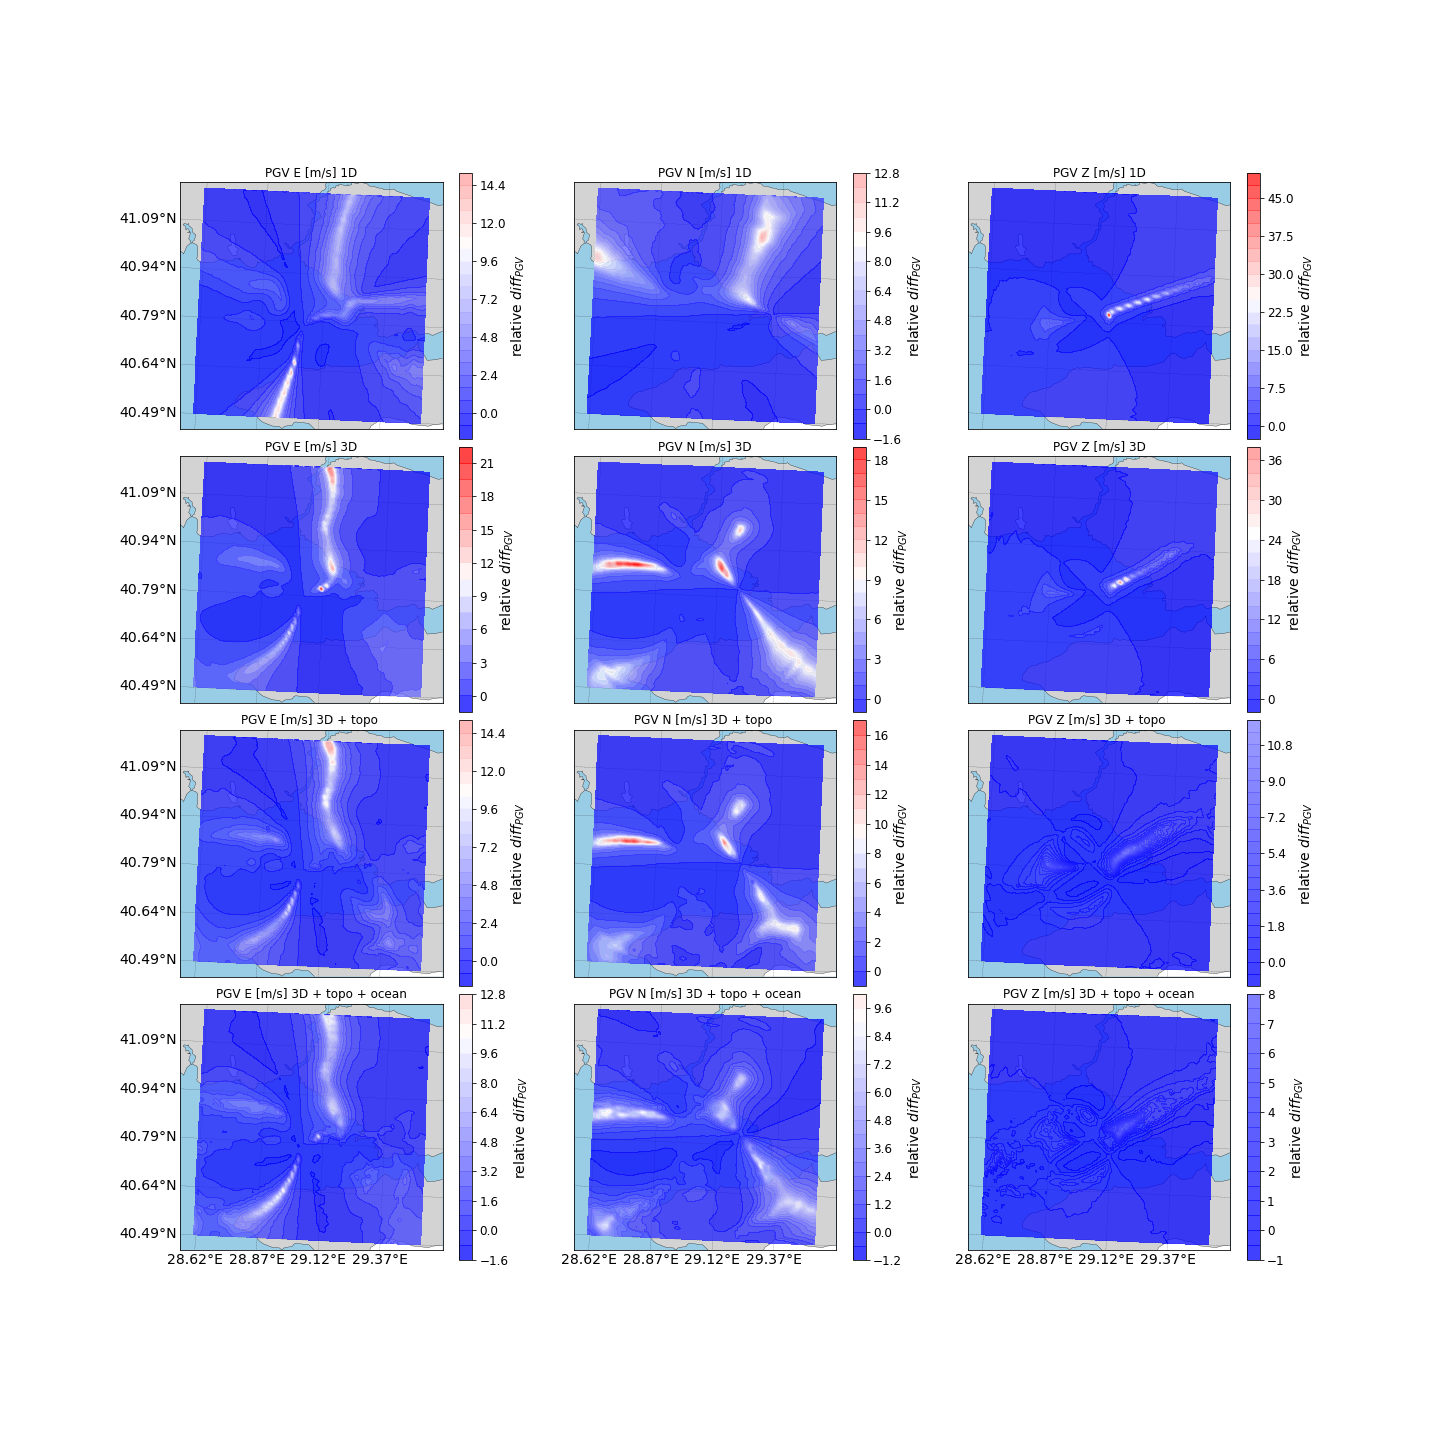
\includegraphics[width=1\linewidth,trim = 2cm 5cm 1cm 5cm, clip]{images_results/strike_variation_epsilon25_sc2.png}
    \caption{CMT2 relative difference between CMT with a strike variation of 22.5$\degree$ with respect to the reference scenario. Colourbar set to the total minima and maxima of the 11.25$\degree$ and 22.5$\degree$ plots for comparison.}
    \label{fig:ref_eps25-2}
\end{figure}

\subsubsection{CMT3}

\begin{figure}
    \centering
    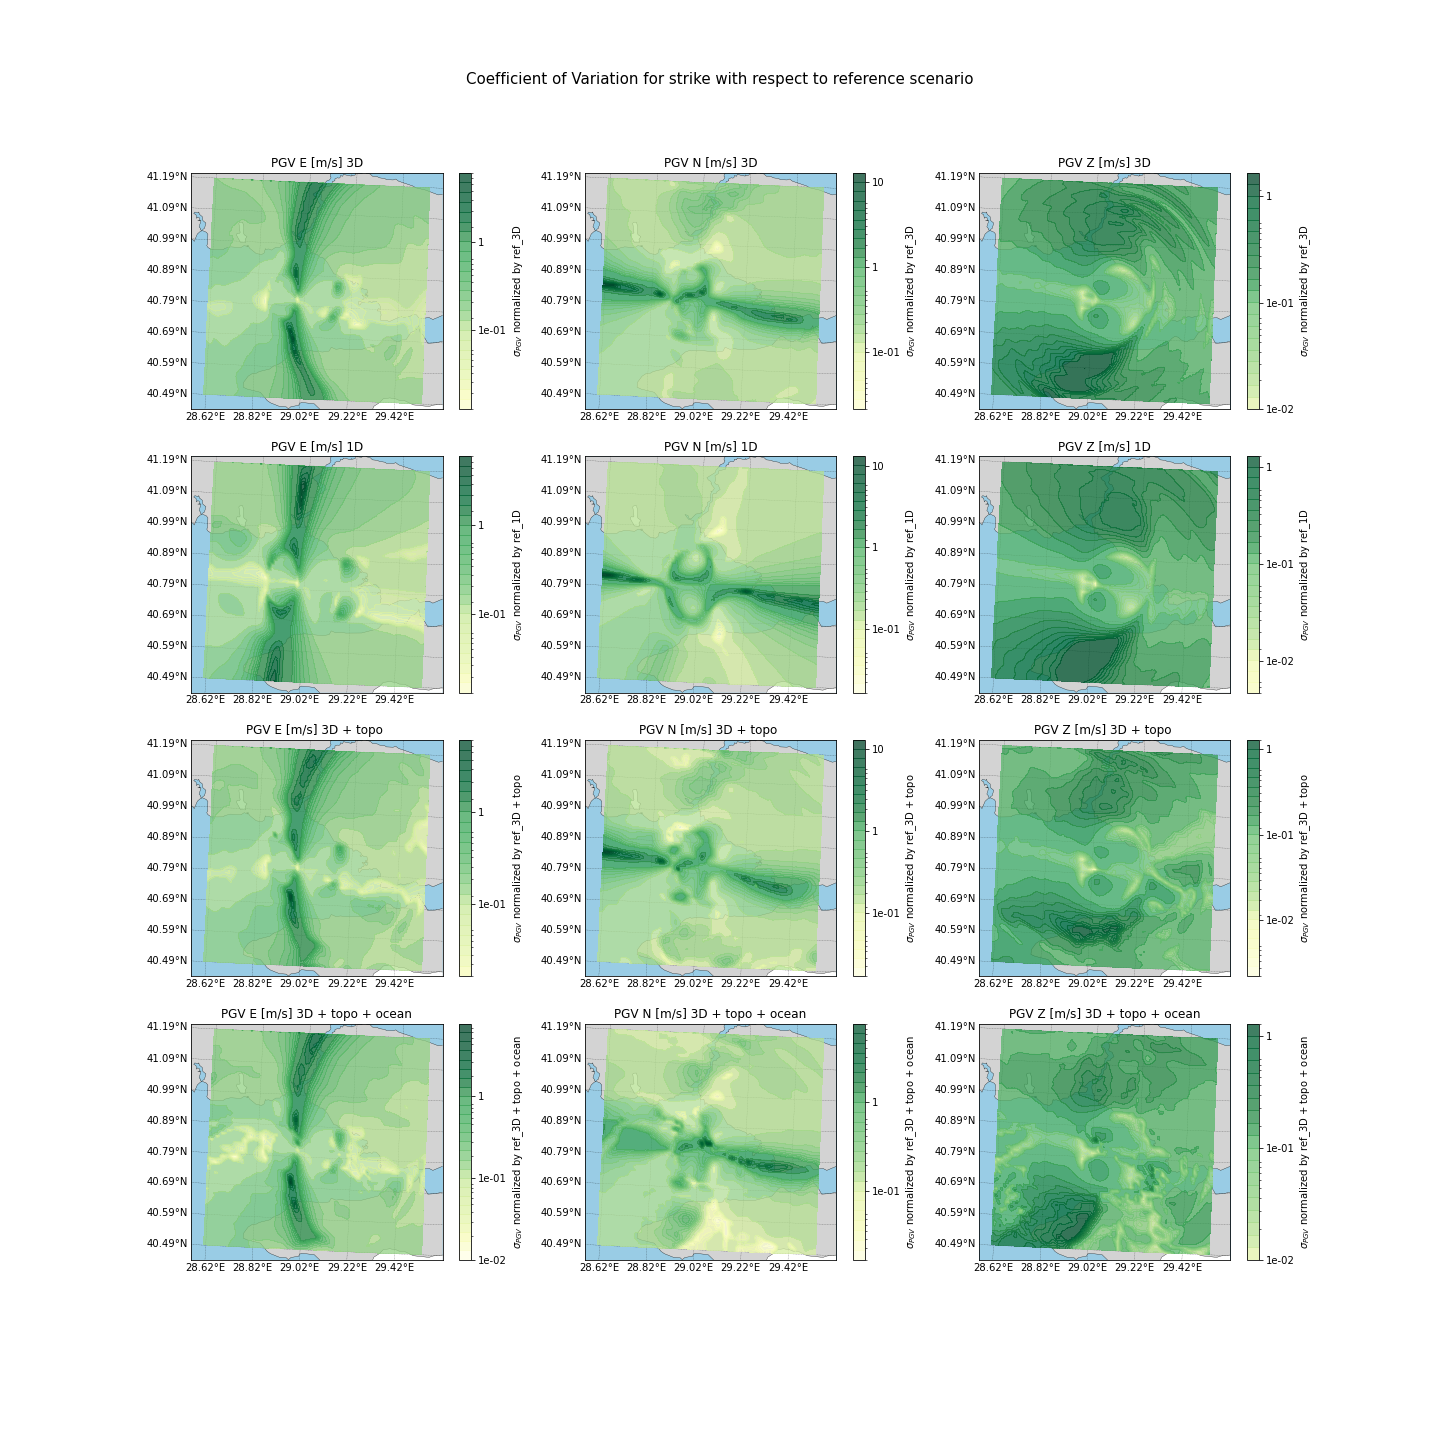
\includegraphics[width=1\linewidth]{images_results/strike_variation_sigma_sc3.png}
    \caption{CMT2 coefficient of variation $Cv$ of strike variation, for each model domain in E, N and Z direction. Colourbar set to logarithmic to adequately show the large differences.}
    \label{fig:cmt2sigm}
\end{figure}


\begin{figure}[!h]
    \centering
    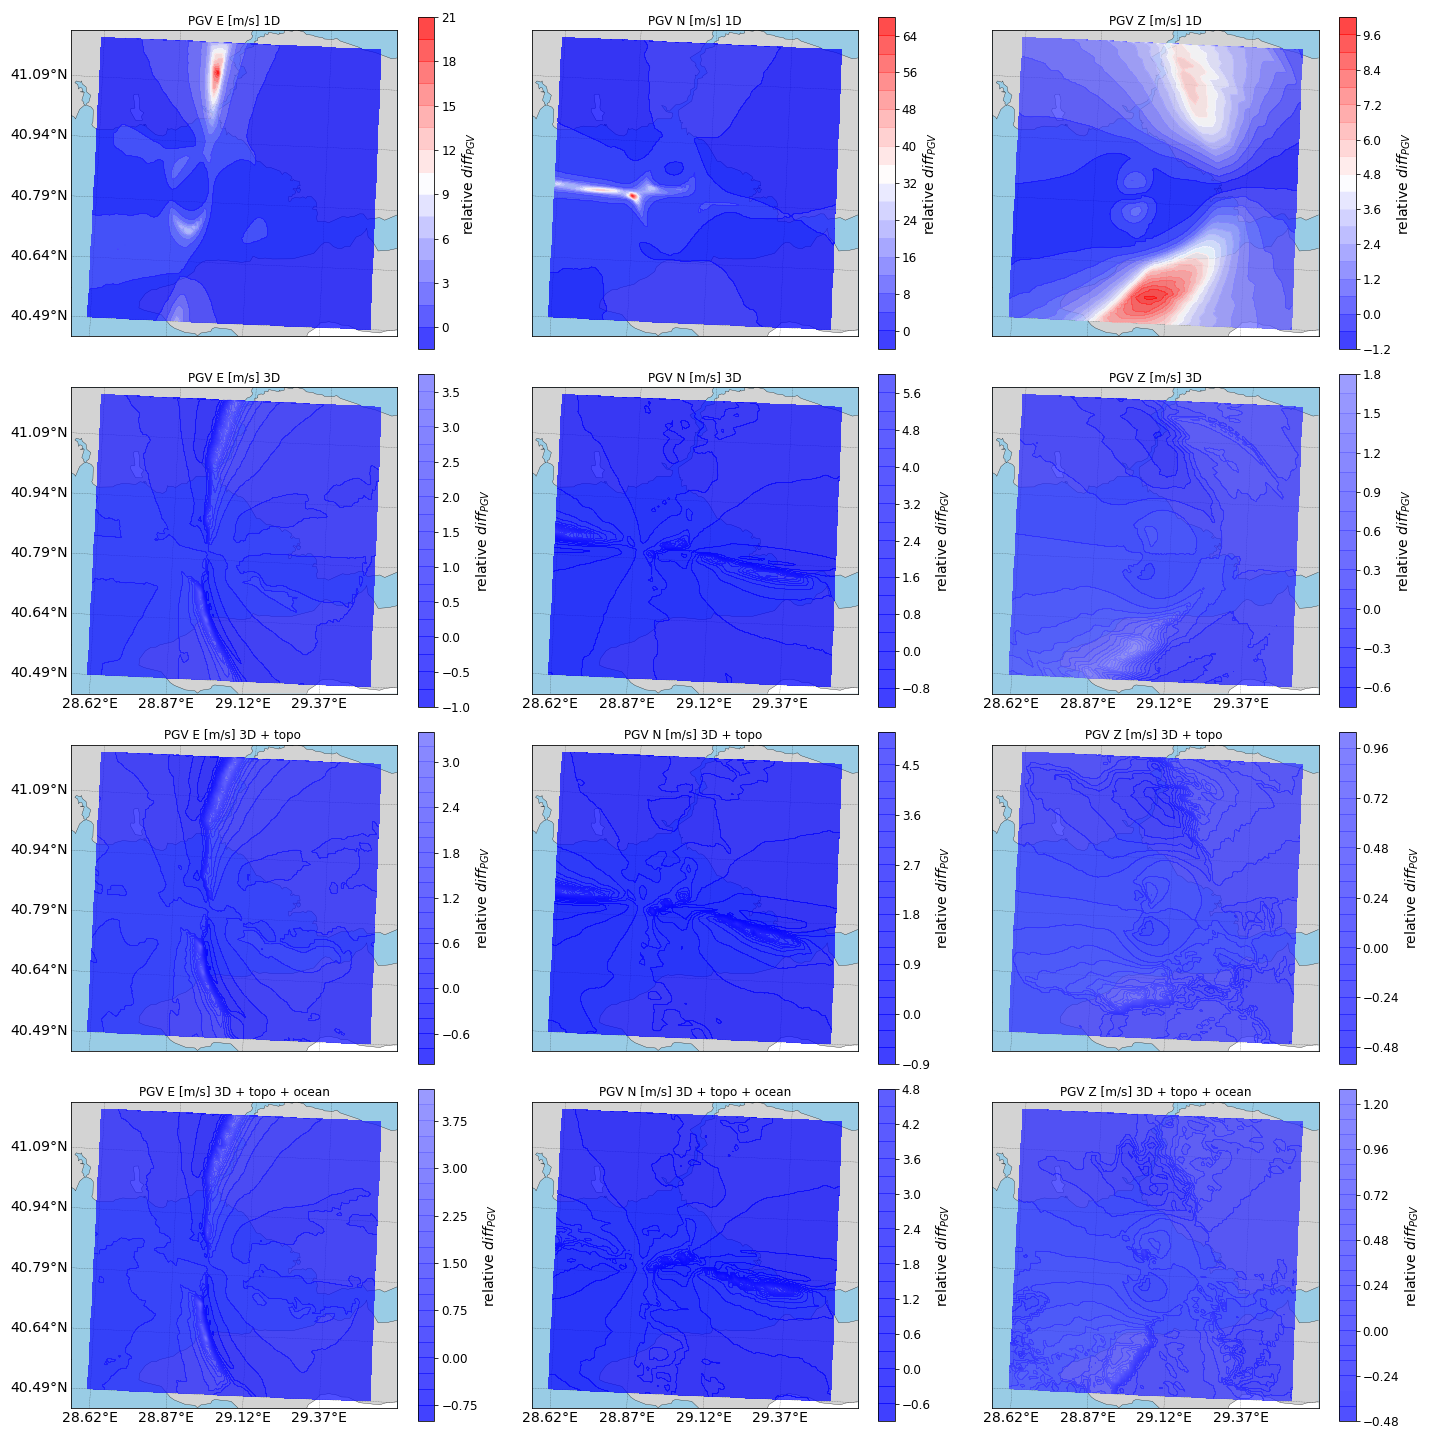
\includegraphics[width=1\linewidth]{images_results/strike_variation_epsilon12_sc3.png}
    \caption{CMT3 relative difference between a scenario with a strike variation of 11.25$\degree$ with respect to the reference scenario. Colourbar set to the total minima and maxima of the 11.25$\degree$ and 22.5$\degree$ plots for comparison.}
    \label{fig:ref_eps12-2}
\end{figure}

\begin{figure}[!h]
    \centering
    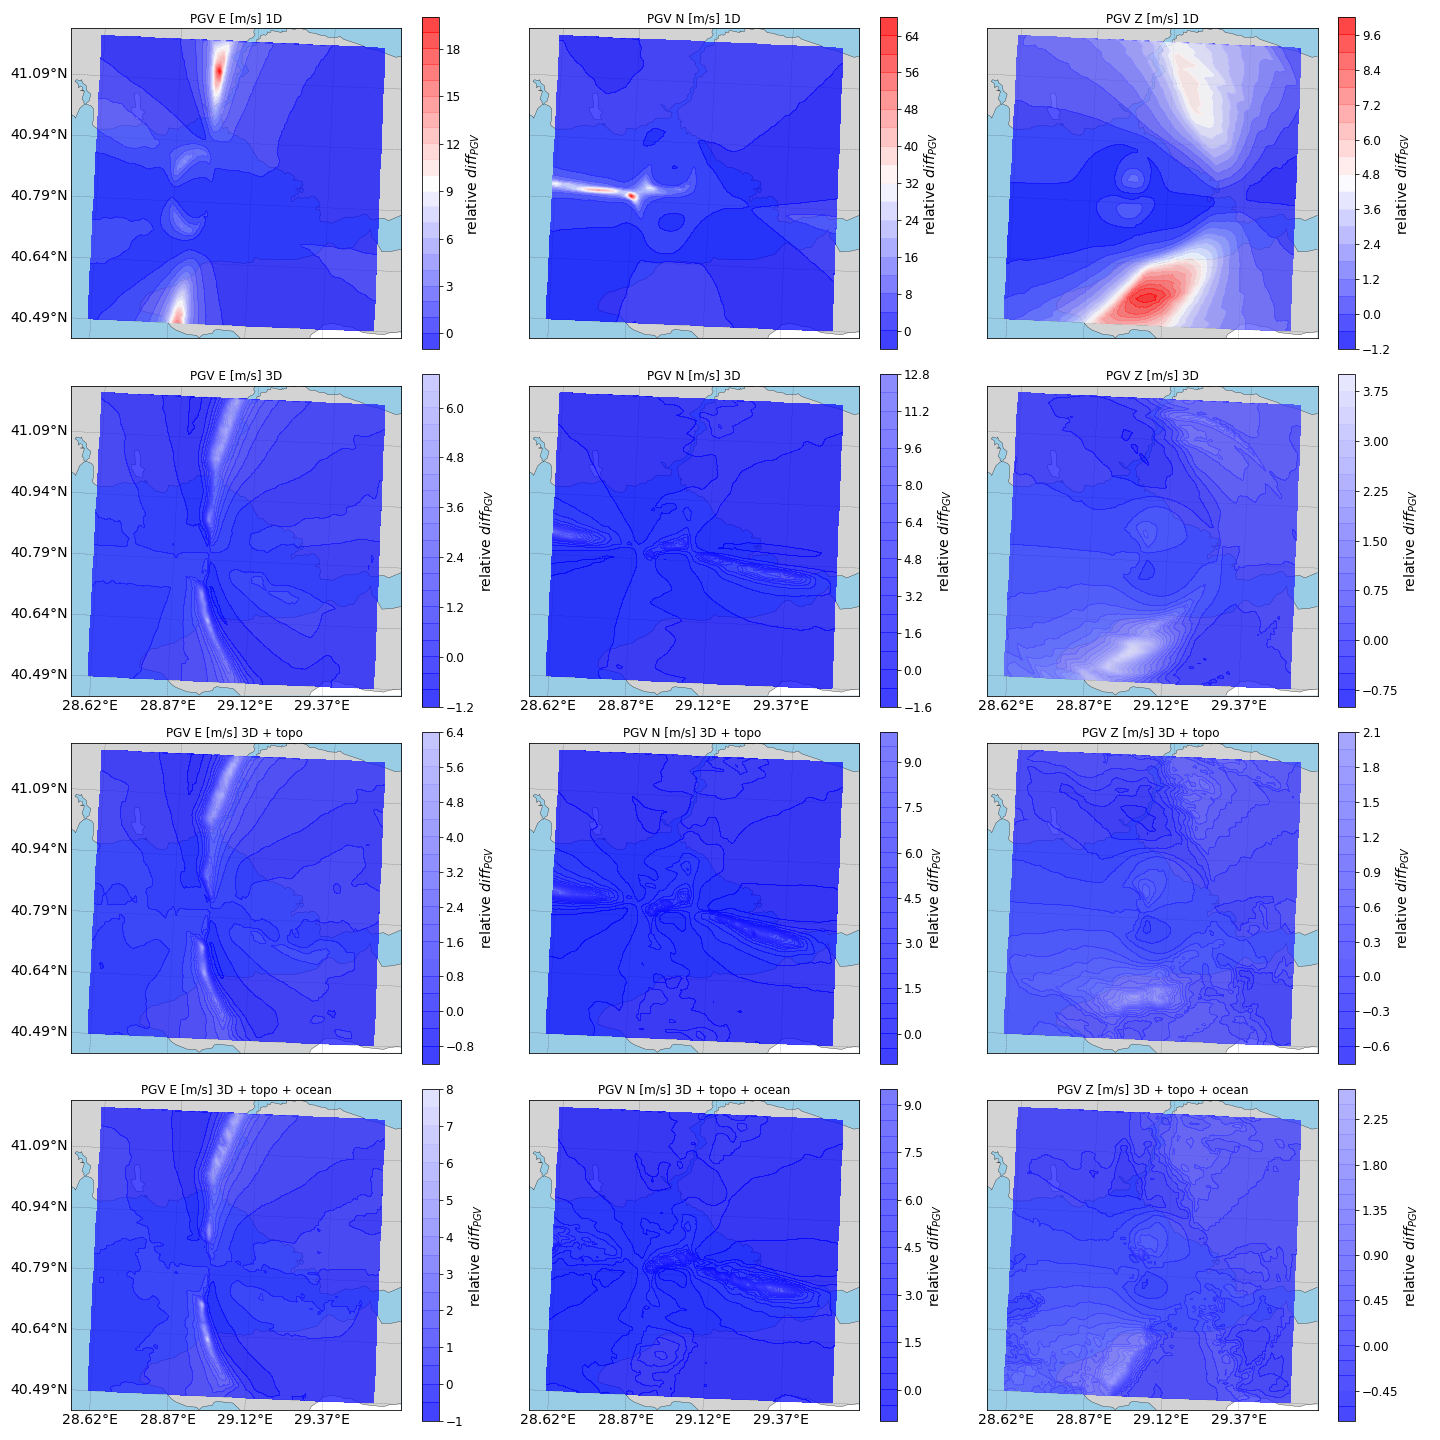
\includegraphics[width=1\linewidth]{images_results/strike_variation_epsilon25_sc3.png}
    \caption{CMT3 relative difference between CMT with a strike variation of 22.5$\degree$ with respect to the reference scenario. Colourbar set to the total minima and maxima of the 11.25$\degree$ and 22.5$\degree$ plots for comparison.}
    \label{fig:ref_eps25-2}
\end{figure}

\FloatBarrier

\subsubsection{CMT4}

\begin{figure}[!h]
    \centering
    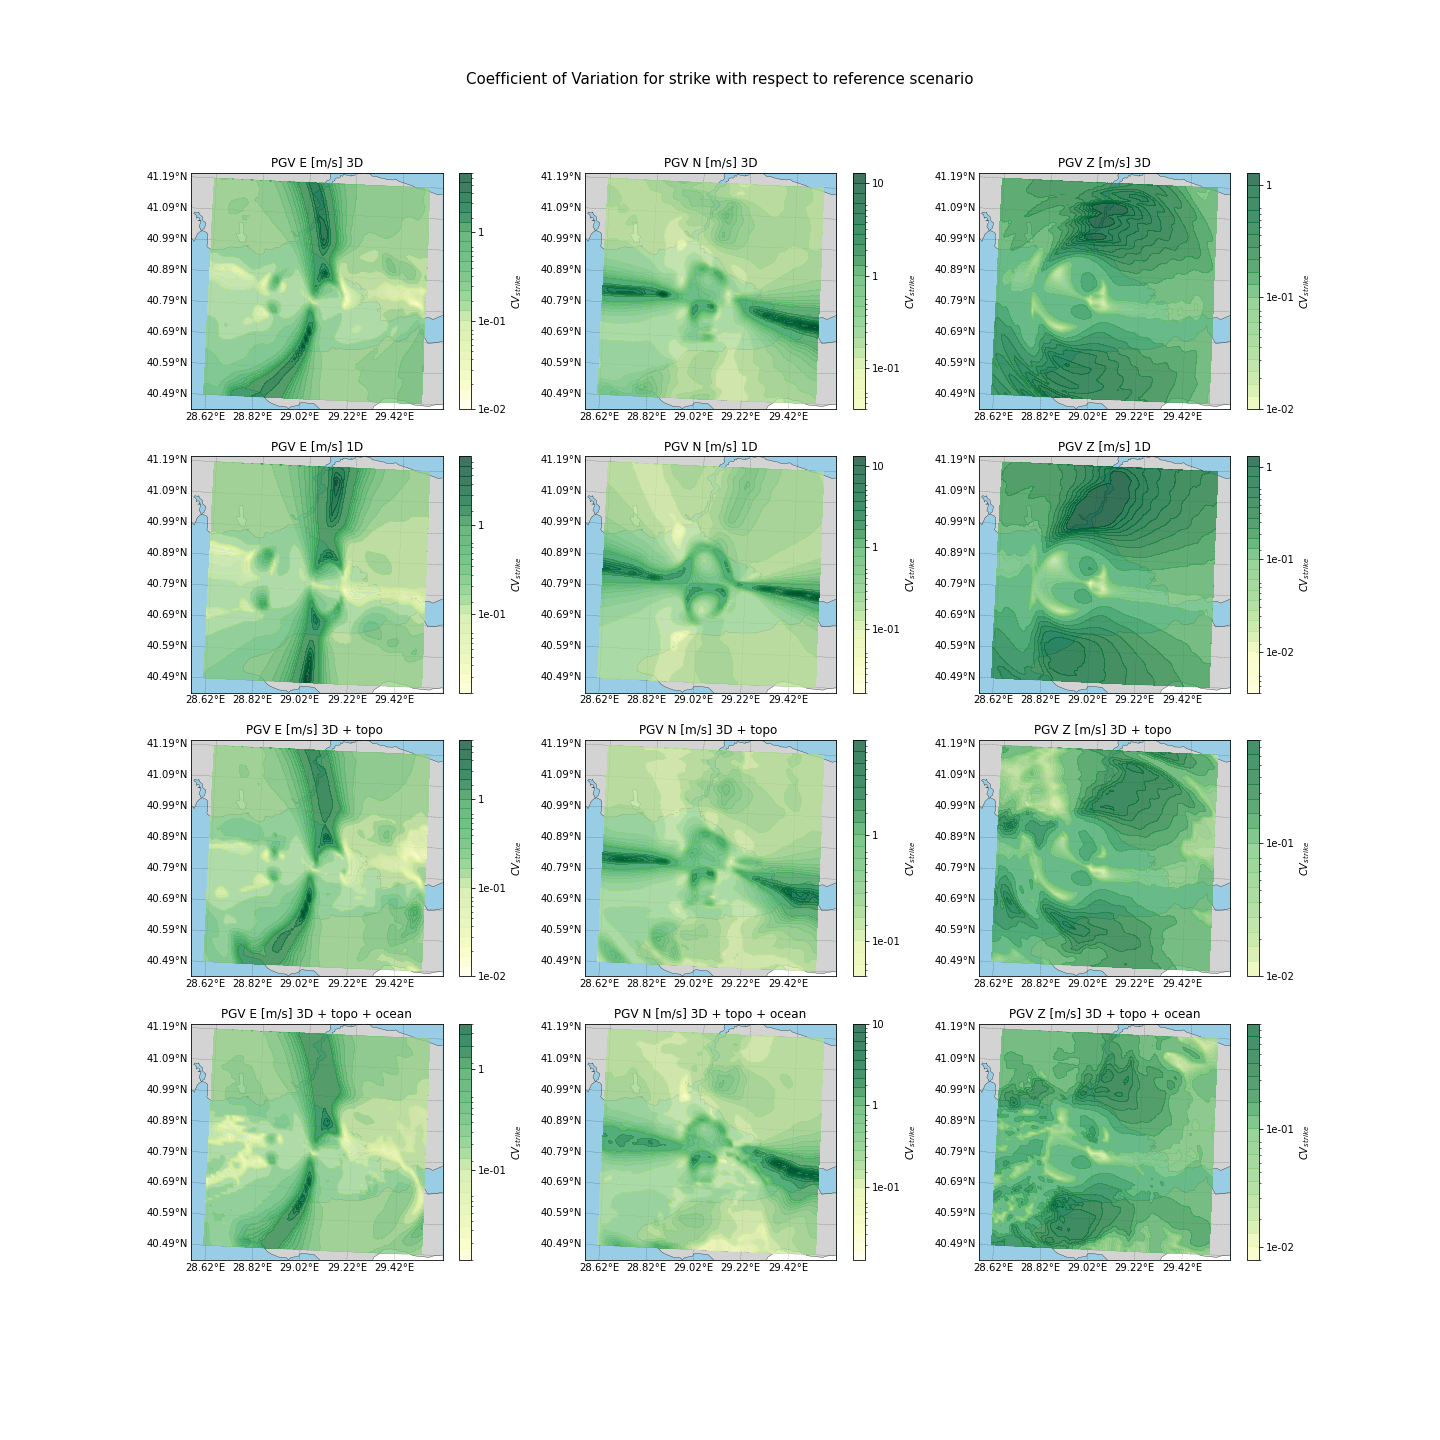
\includegraphics[width=1\linewidth]{images_results/strike_variation_sigma_sc4.png}
    \caption{CMT3 coefficient of variation $Cv$ of strike variation, for each model domain in E, N and Z direction. Colourbar set to logarithmic to adequately show the large differences.}
    \label{fig:cmt3sigm}
\end{figure}

\FloatBarrier

\begin{figure}[!h]
    \centering
    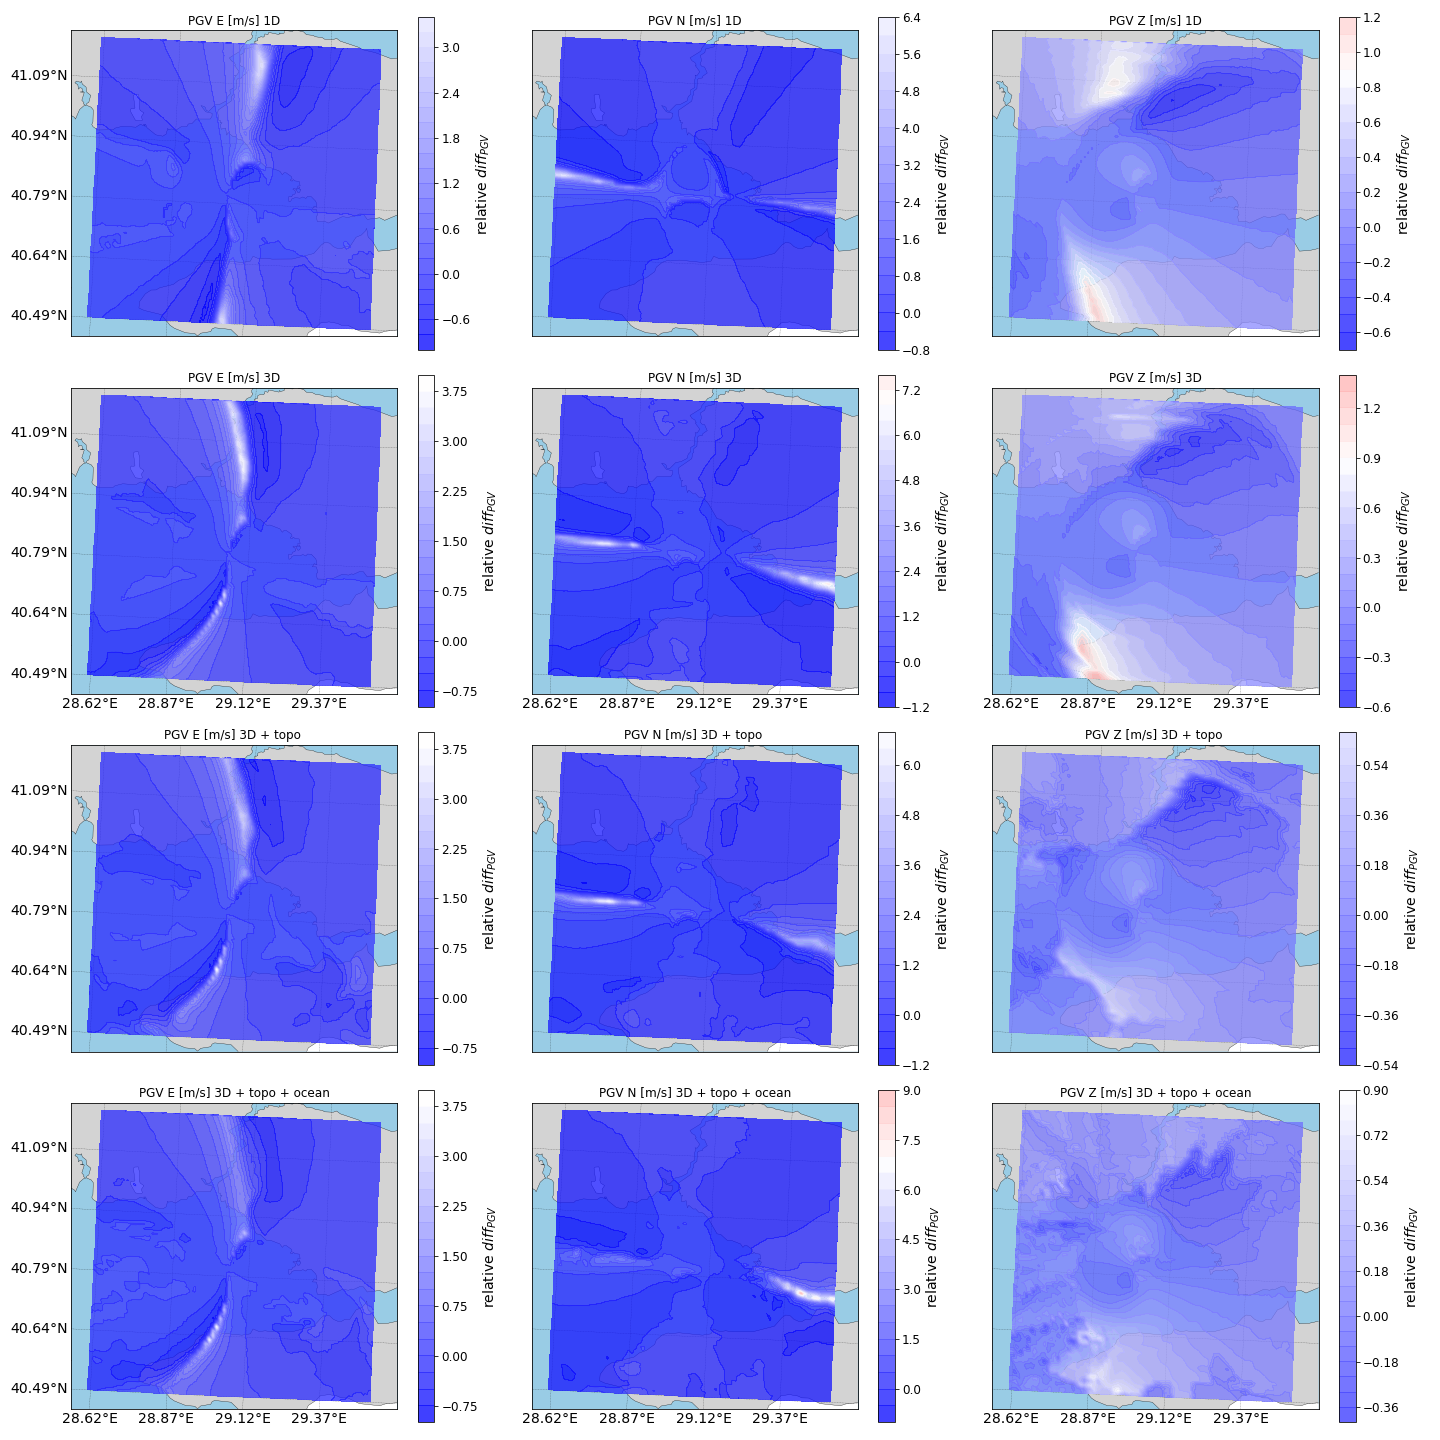
\includegraphics[width=1\linewidth]{images_results/strike_variation_epsilon12_sc4.png}
    \caption{CMT4 relative difference between a scenario with a strike variation of 11.25$\degree$ with respect to the reference scenario. Colourbar set to the total minima and maxima of the 11.25$\degree$ and 22.5$\degree$ plots for comparison.}
    \label{fig:ref_eps12-2}
\end{figure}

\FloatBarrier

\begin{figure}[!h]
    \centering
    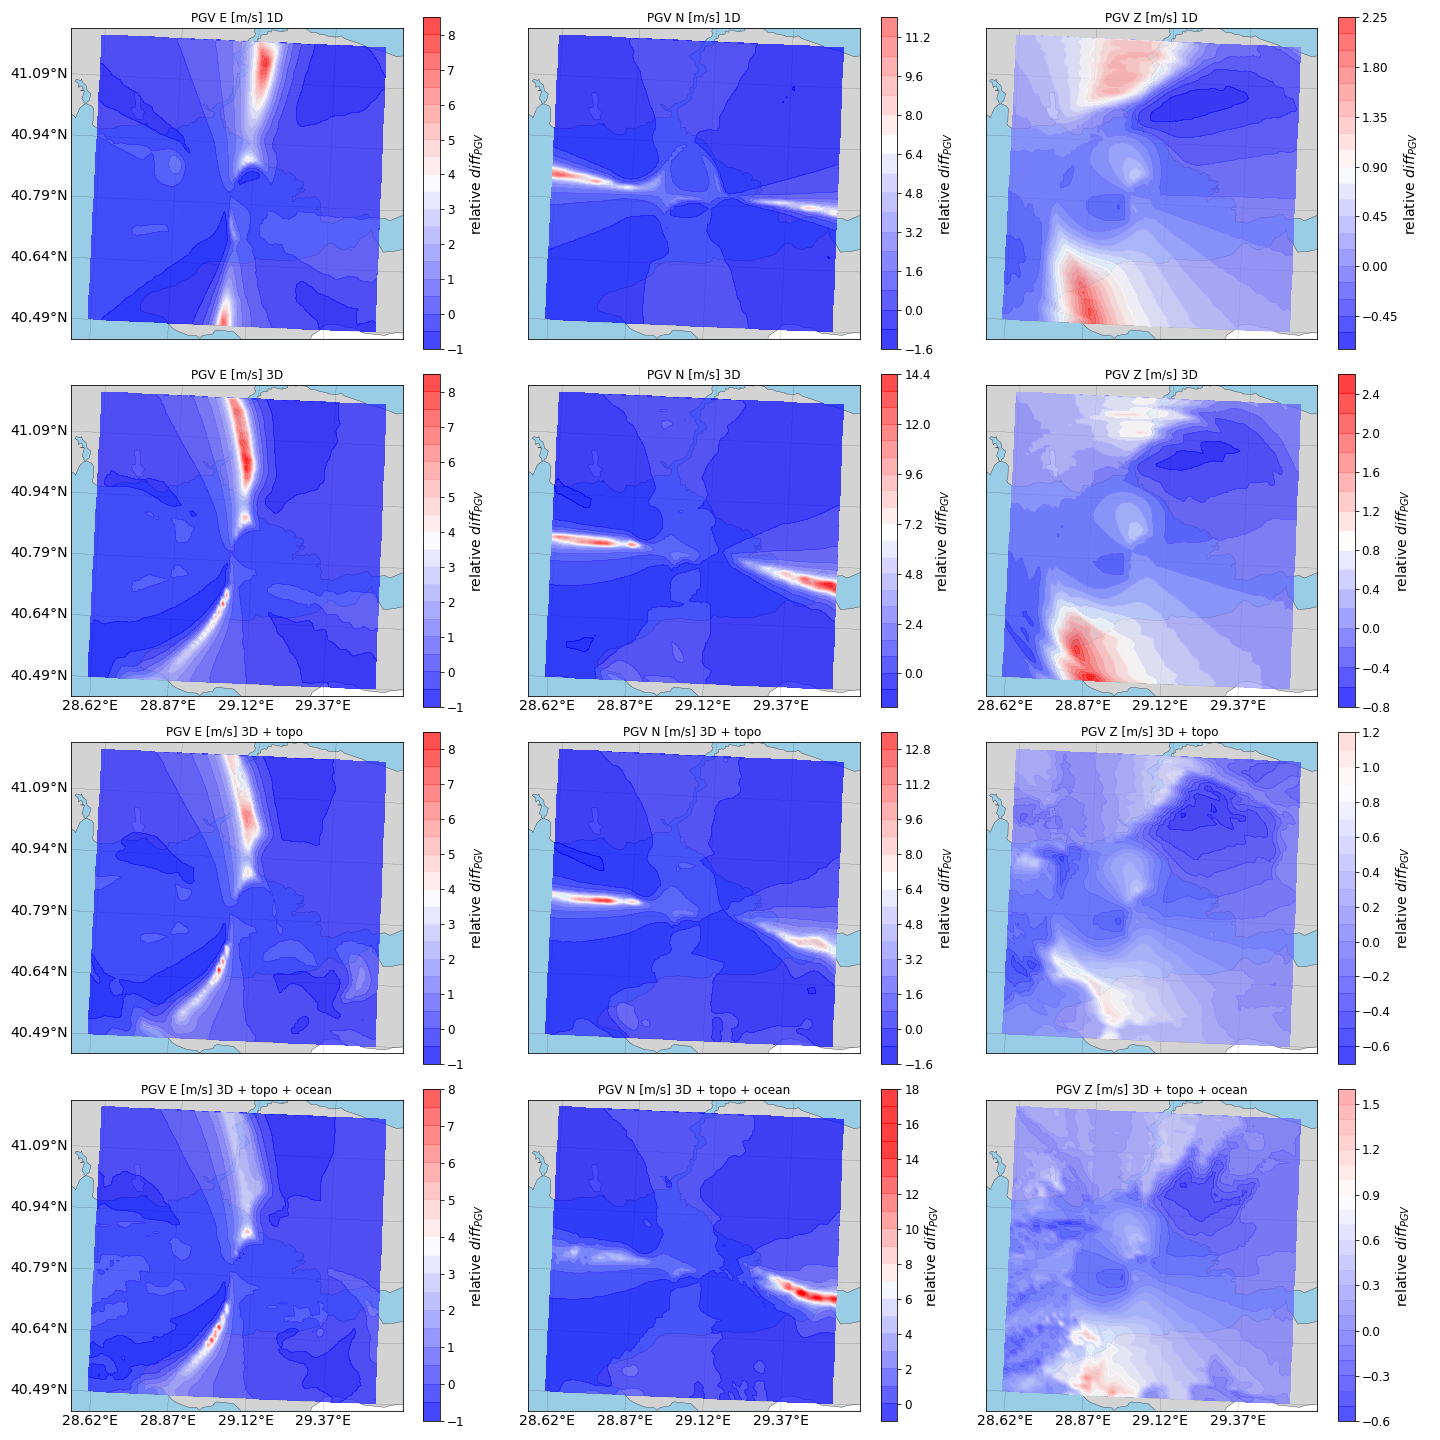
\includegraphics[width=1\linewidth]{images_results/strike_variation_epsilon25_sc4.png}
    \caption{CMT4 relative difference between a scenario with a strike variation of 22.5$\degree$ with respect to the reference scenario. Colourbar set to the total minima and maxima of the 11.25$\degree$ and 22.5$\degree$ plots for comparison.}
    \label{fig:ref_eps25-2}
\end{figure}

\FloatBarrier

\subsection{Variation dip figures CMT3 and CMT4}

\subsubsection{CMT2}

\begin{figure}
    \centering
    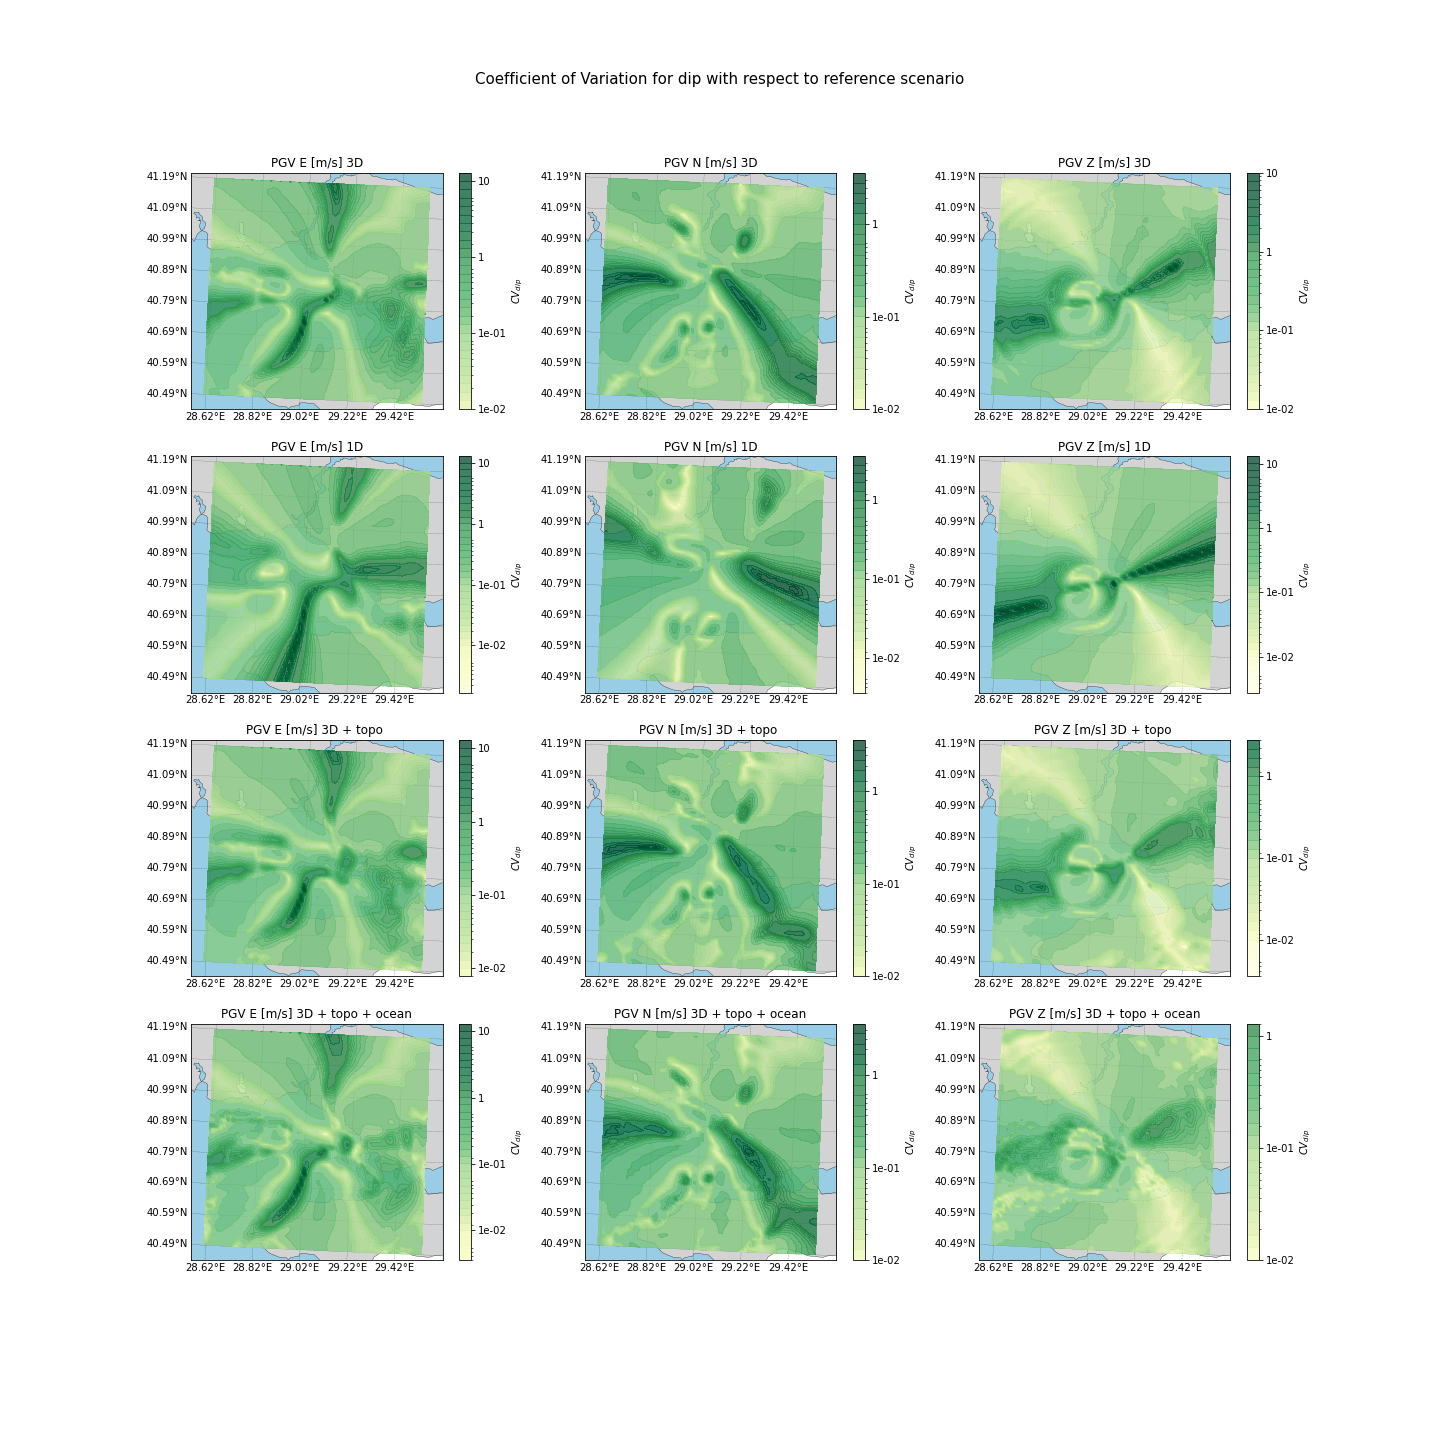
\includegraphics[width=1\linewidth,trim = 2cm 5cm 1cm 5cm, clip]{images_results/dip_variation_sigma_sc2.png}
    \caption{CMT2 coefficient of variation $Cv$ of dip variation, for each model domain in E, N and Z direction. Colourbar set to logarithmic to adequately show the large differences.}
    \label{fig:cmt2sigm}
\end{figure}


\begin{figure}[!h]
    \centering
    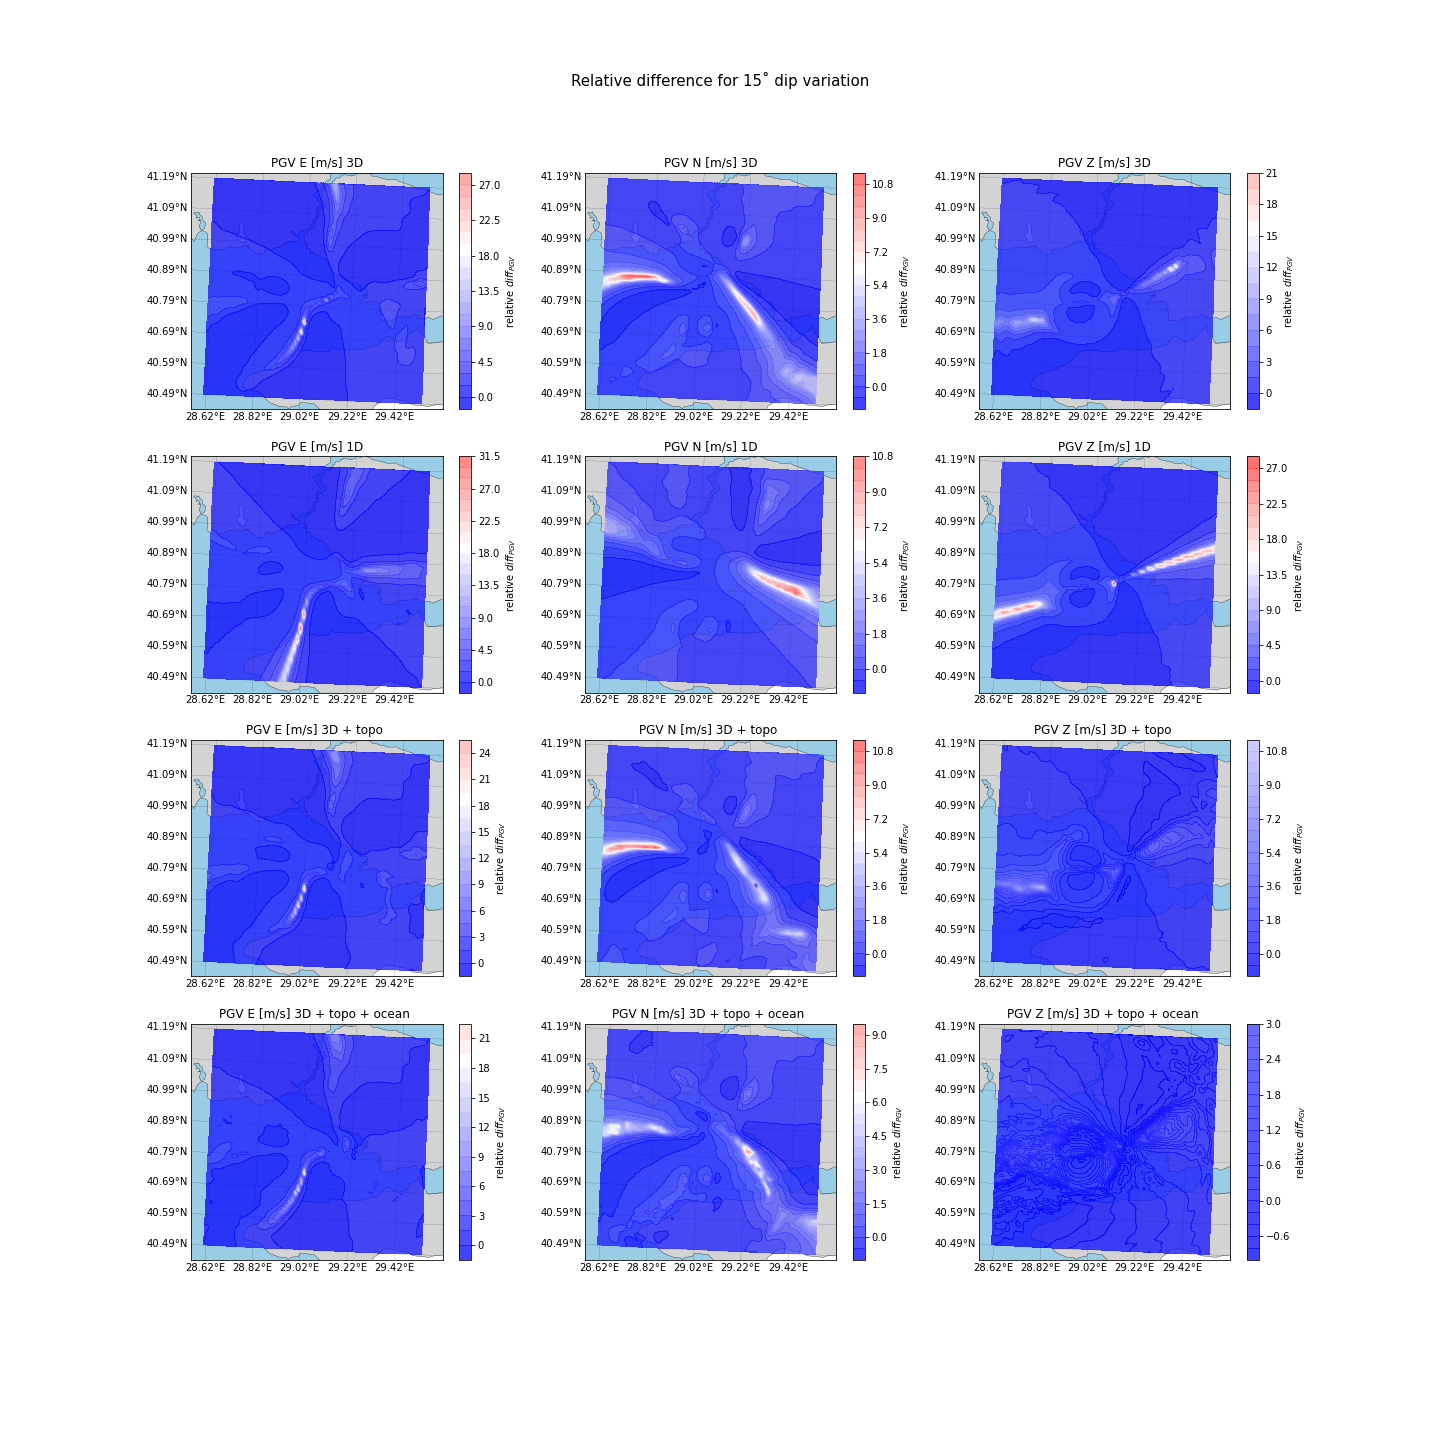
\includegraphics[width=1\linewidth,trim = 2cm 5cm 1cm 5cm, clip]{images_results/dip_variation_epsilon12_sc2.png}
    \caption{CMT3 relative difference between a scenario with a dip variation of 11.25$\degree$ with respect to the reference scenario. Colourbar set to the total minima and maxima of the 11.25$\degree$ and 22.5$\degree$ plots for comparison.}
    \label{fig:ref_eps12-2}
\end{figure}

\begin{figure}[!h]
    \centering
    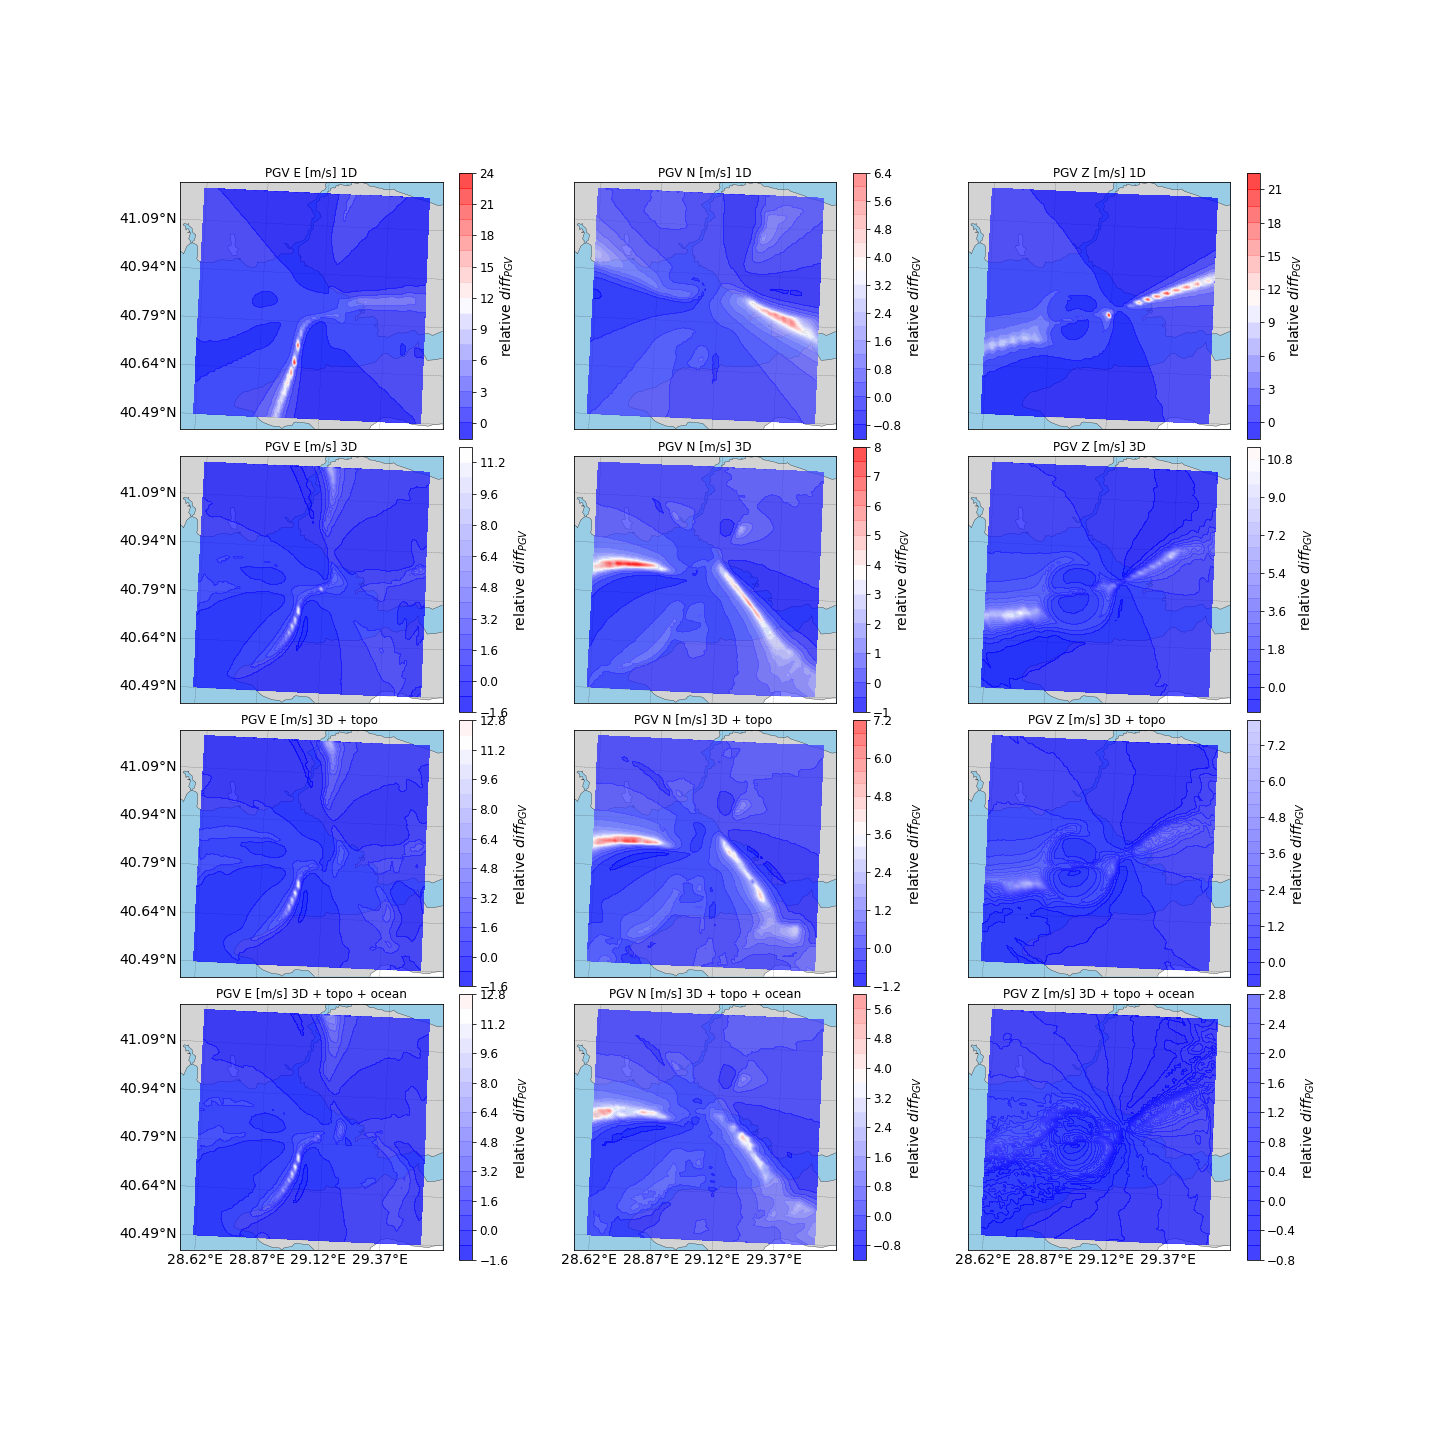
\includegraphics[width=1\linewidth,trim = 2cm 5cm 1cm 5cm, clip]{images_results/dip_variation_epsilon25_sc2.png}
    \caption{CMT3 relative difference between CMT with a dip variation of 22.5$\degree$ with respect to the reference scenario. Colourbar set to the total minima and maxima of the 11.25$\degree$ and 22.5$\degree$ plots for comparison.}
    \label{fig:ref_eps25-2}
\end{figure}

\subsubsection{CMT3}

\begin{figure}
    \centering
    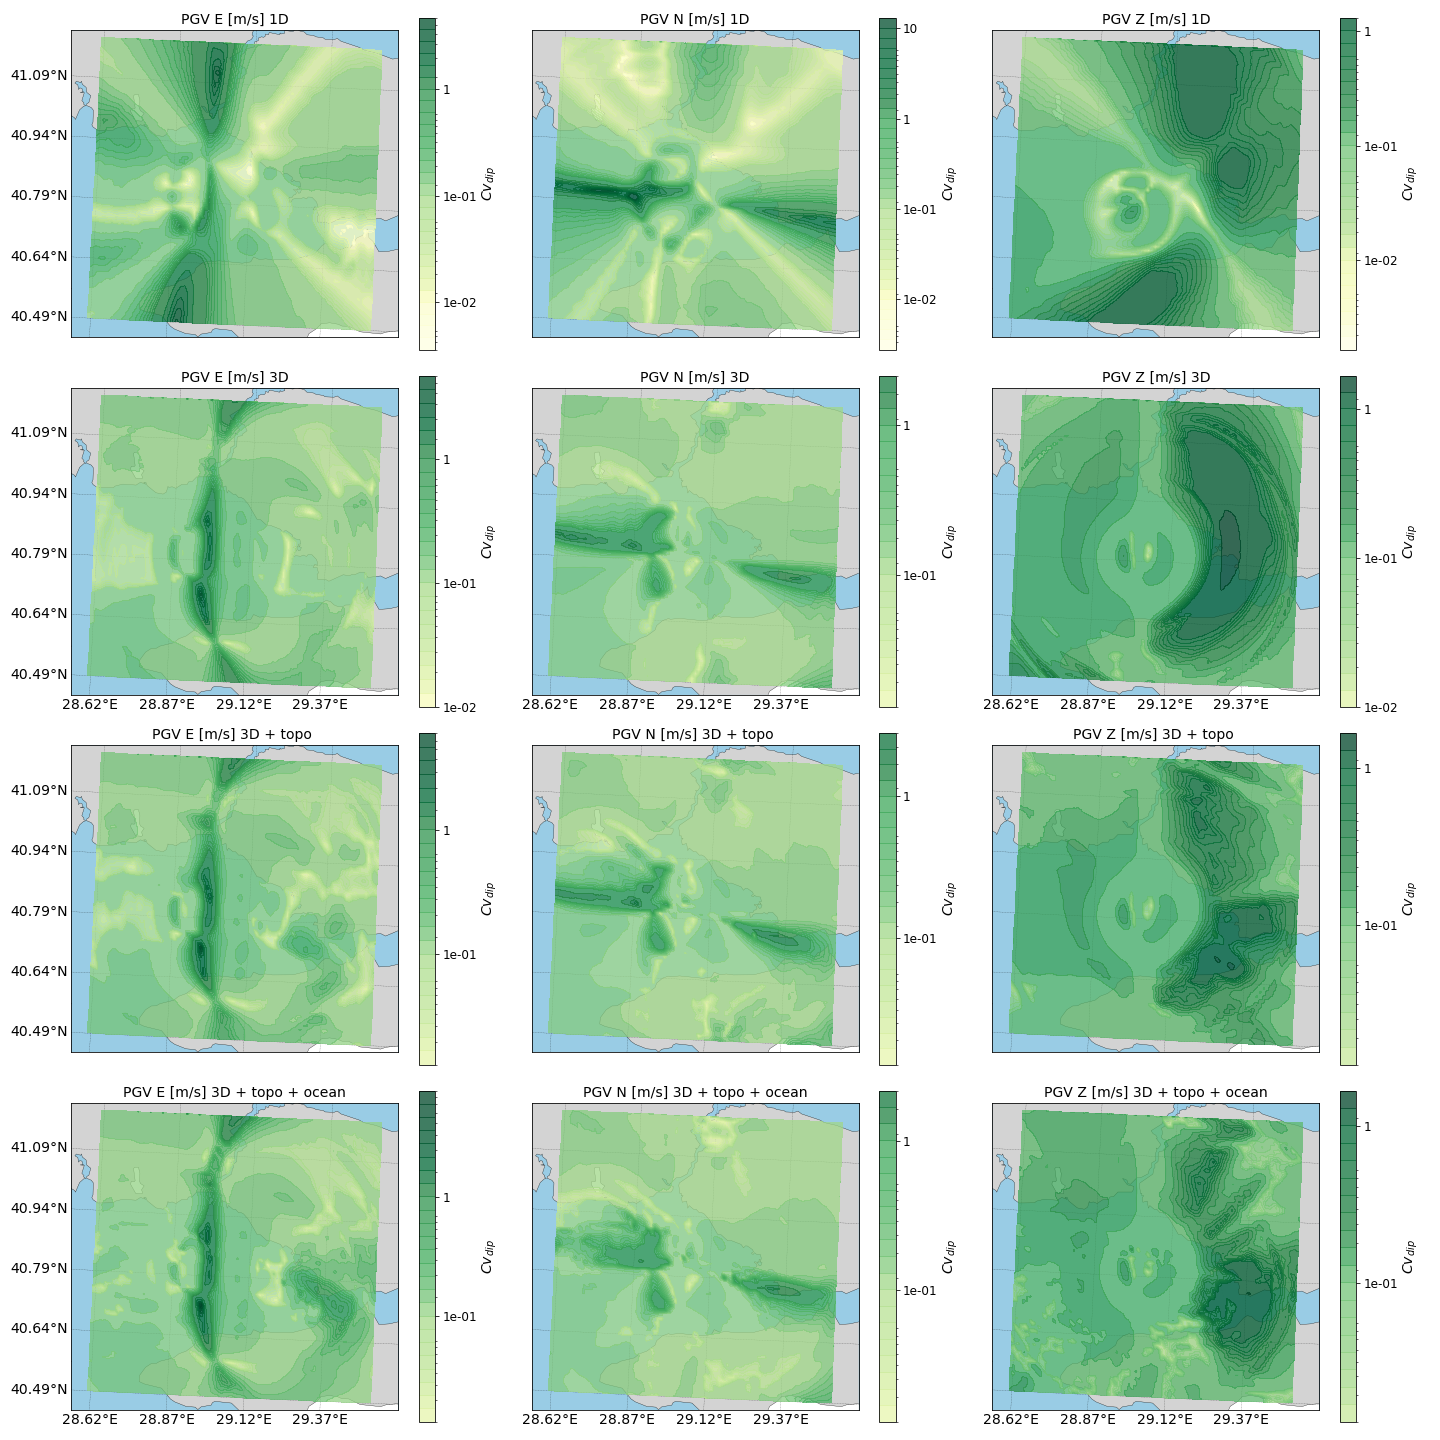
\includegraphics[width=1\linewidth,trim = 2cm 5cm 1cm 5cm, clip]{images_results/dip_variation_sigma_sc3.png}
    \caption{CMT3 coefficient of variation $Cv$ of dip variation, for each model domain in E, N and Z direction. Colourbar set to logarithmic to adequately show the large differences.}
    \label{fig:cmt2sigm}
\end{figure}


\begin{figure}[!h]
    \centering
    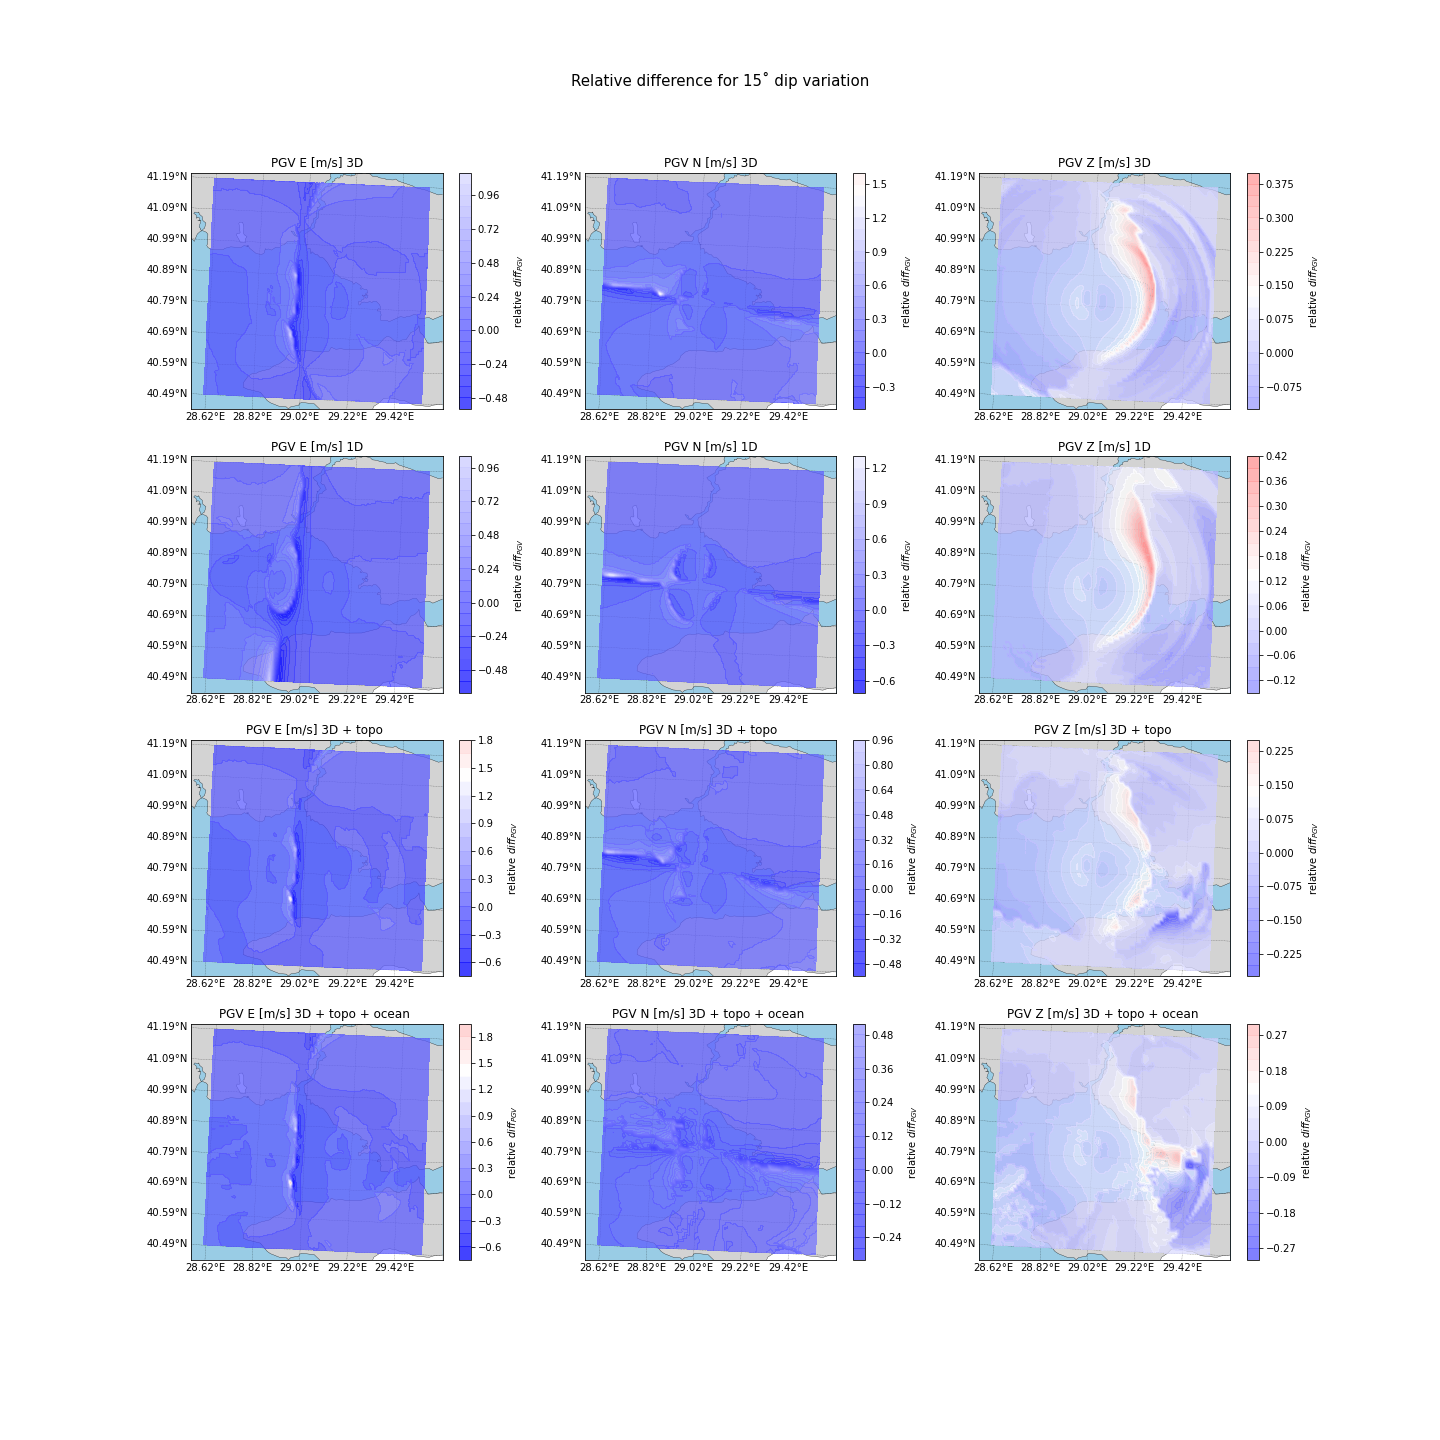
\includegraphics[width=1\linewidth,trim = 2cm 5cm 1cm 5cm, clip]{images_results/dip_variation_epsilon12_sc3.png}
    \caption{CMT3 relative difference between a scenario with a dip variation of 11.25$\degree$ with respect to the reference scenario. Colourbar set to the total minima and maxima of the 11.25$\degree$ and 22.5$\degree$ plots for comparison.}
    \label{fig:ref_eps12-2}
\end{figure}

\begin{figure}[!h]
    \centering
    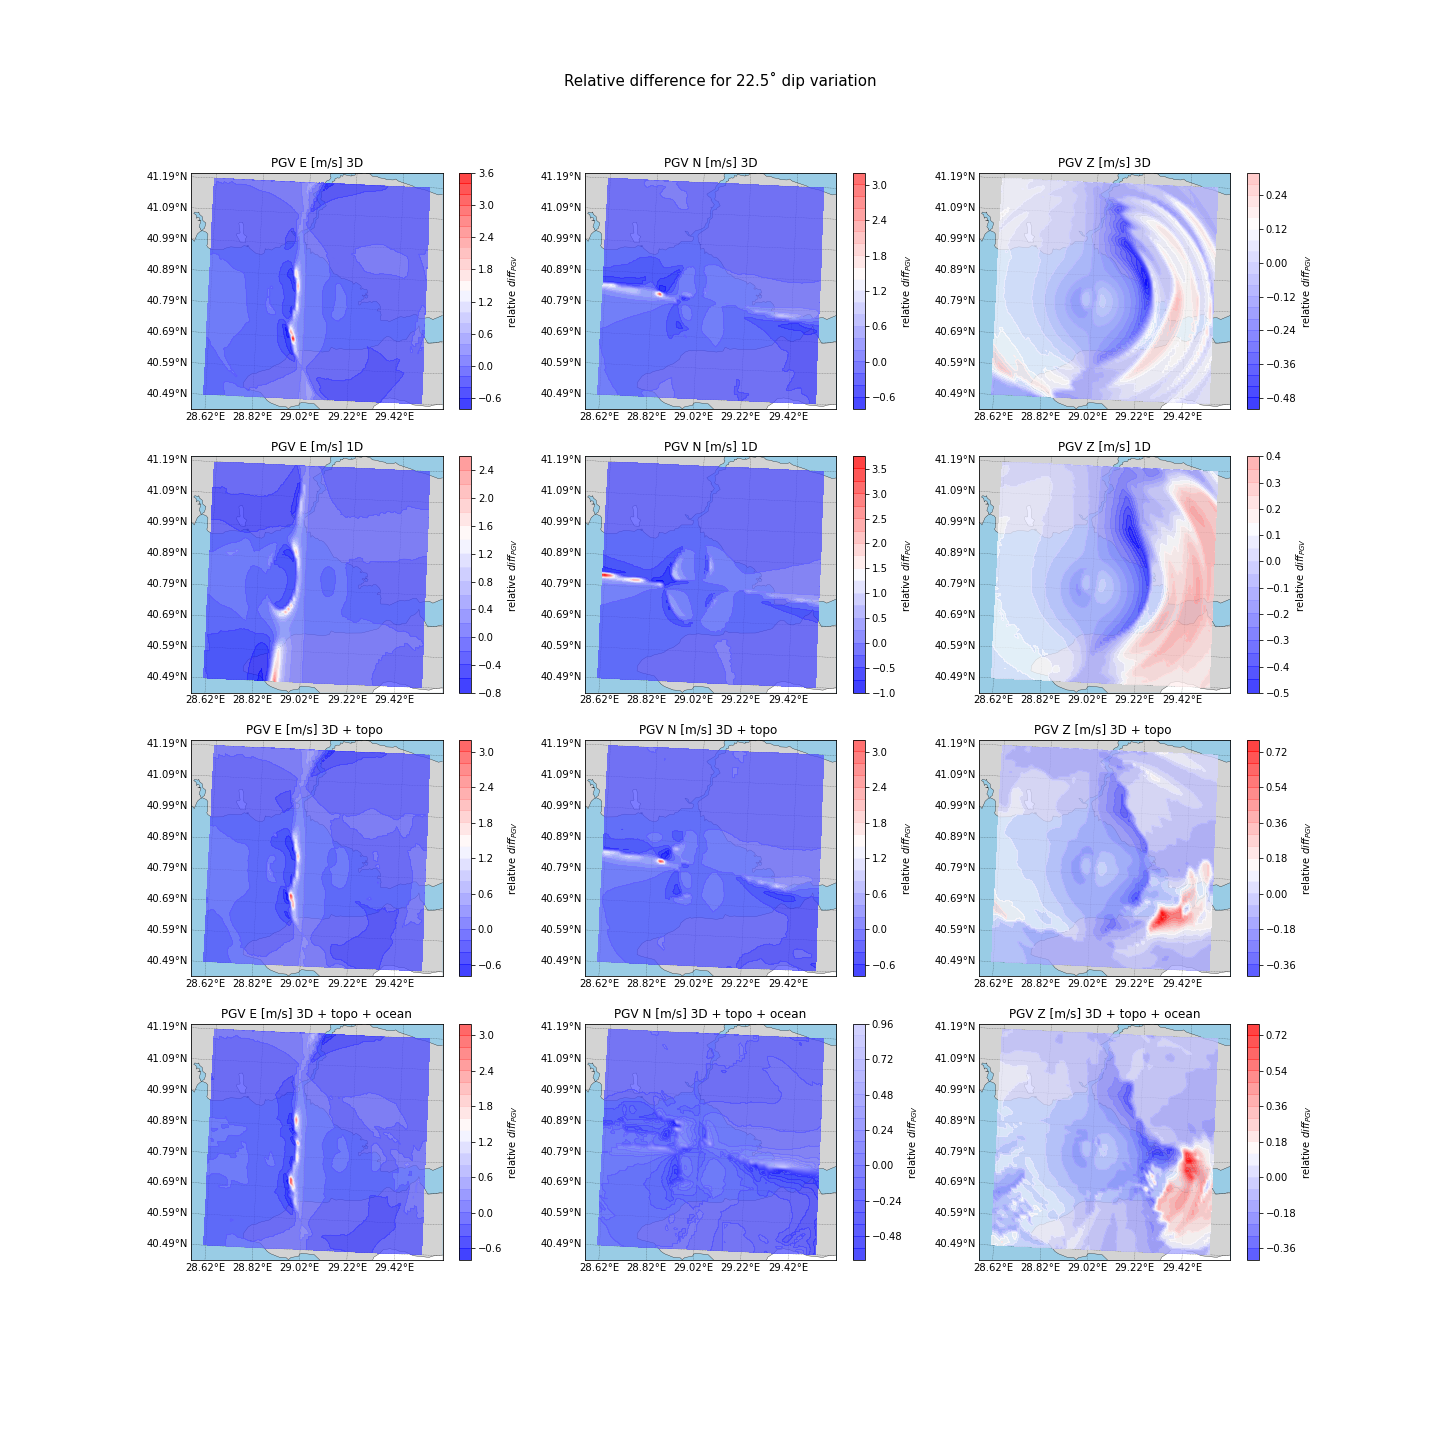
\includegraphics[width=1\linewidth,trim = 2cm 5cm 1cm 5cm, clip]{images_results/dip_variation_epsilon25_sc3.png}
    \caption{CMT3 relative difference between CMT with a dip variation of 22.5$\degree$ with respect to the reference scenario. Colourbar set to the total minima and maxima of the 11.25$\degree$ and 22.5$\degree$ plots for comparison.}
    \label{fig:ref_eps25-2}
\end{figure}

\FloatBarrier

\subsubsection{CMT4}

\begin{figure}[!h]
    \centering
    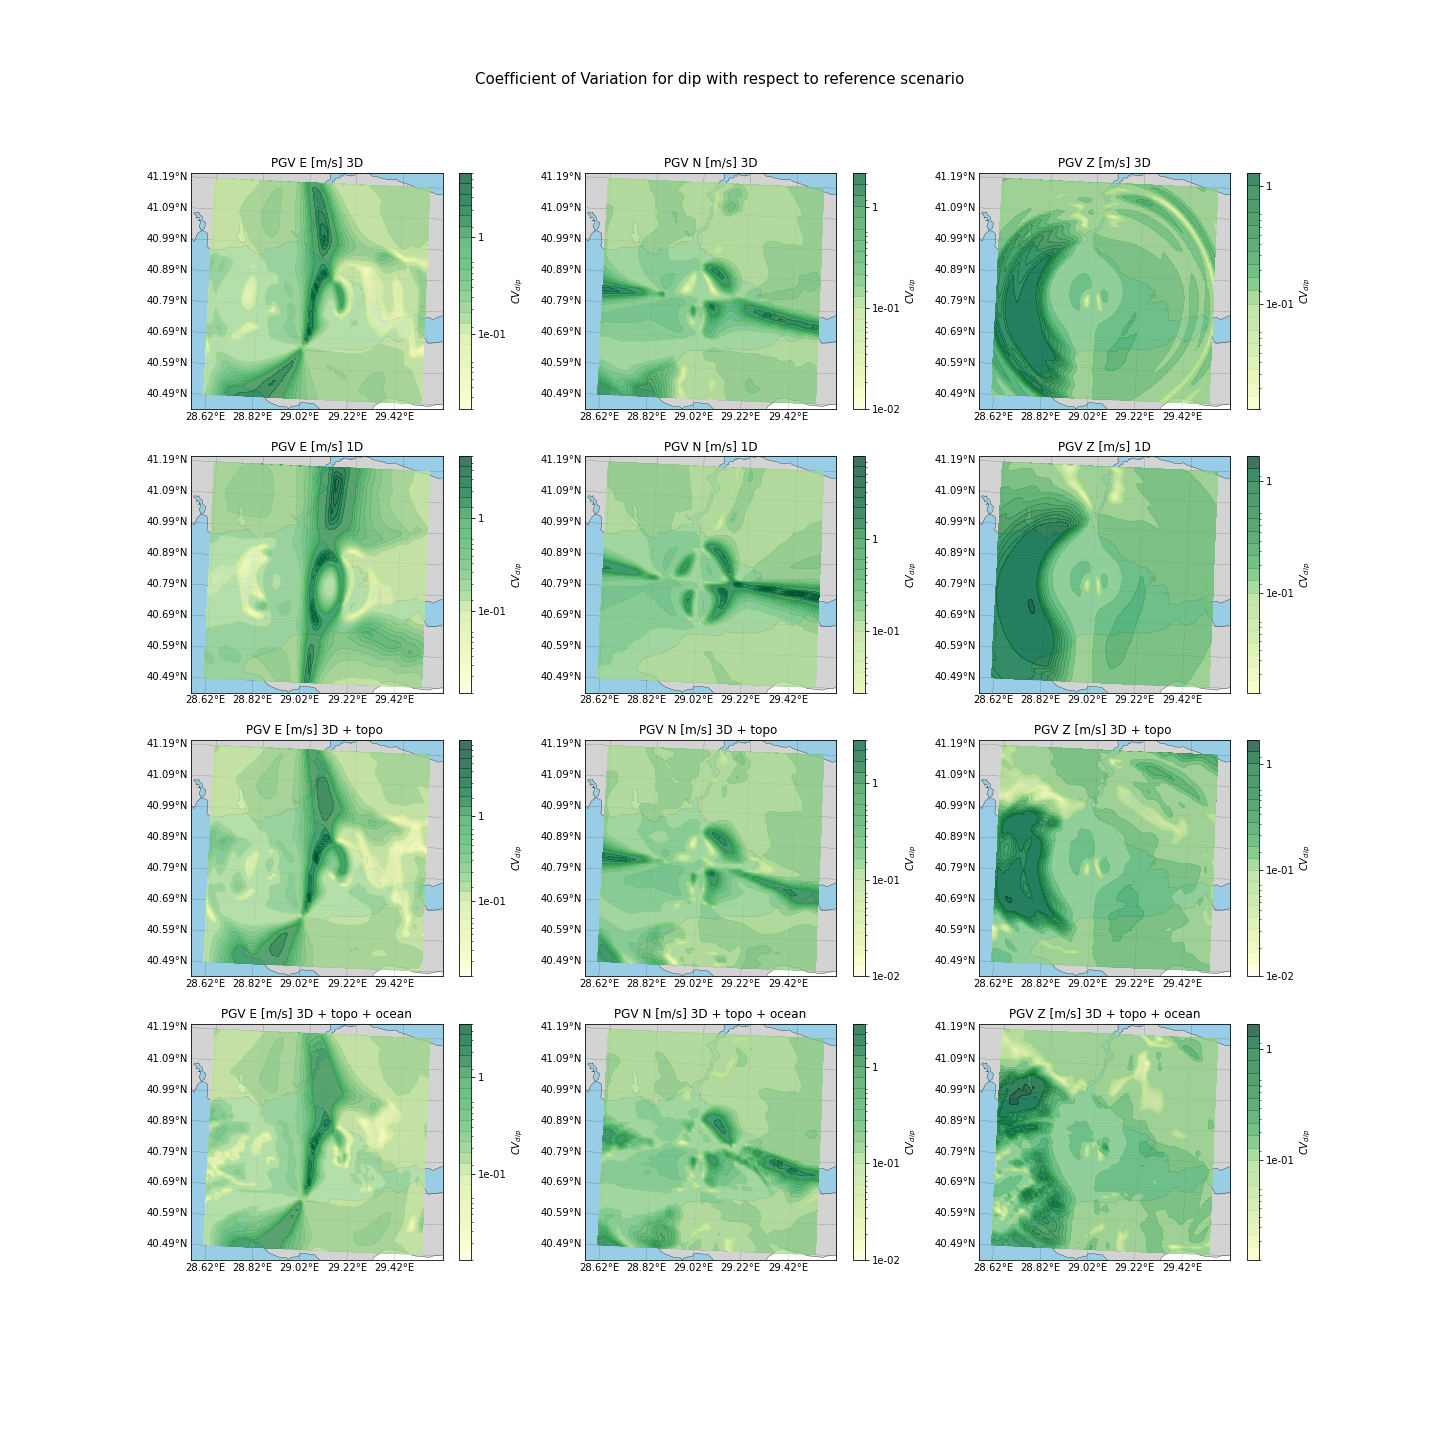
\includegraphics[width=1\linewidth]{images_results/dip_variation_sigma_sc4.png}
    \caption{CMT4 coefficient of variation $Cv$ of dip variation, for each model domain in E, N and Z direction. Colourbar set to logarithmic to adequately show the large differences.}
    \label{fig:cmt3sigm}
\end{figure}

\FloatBarrier

\begin{figure}[!h]
    \centering
    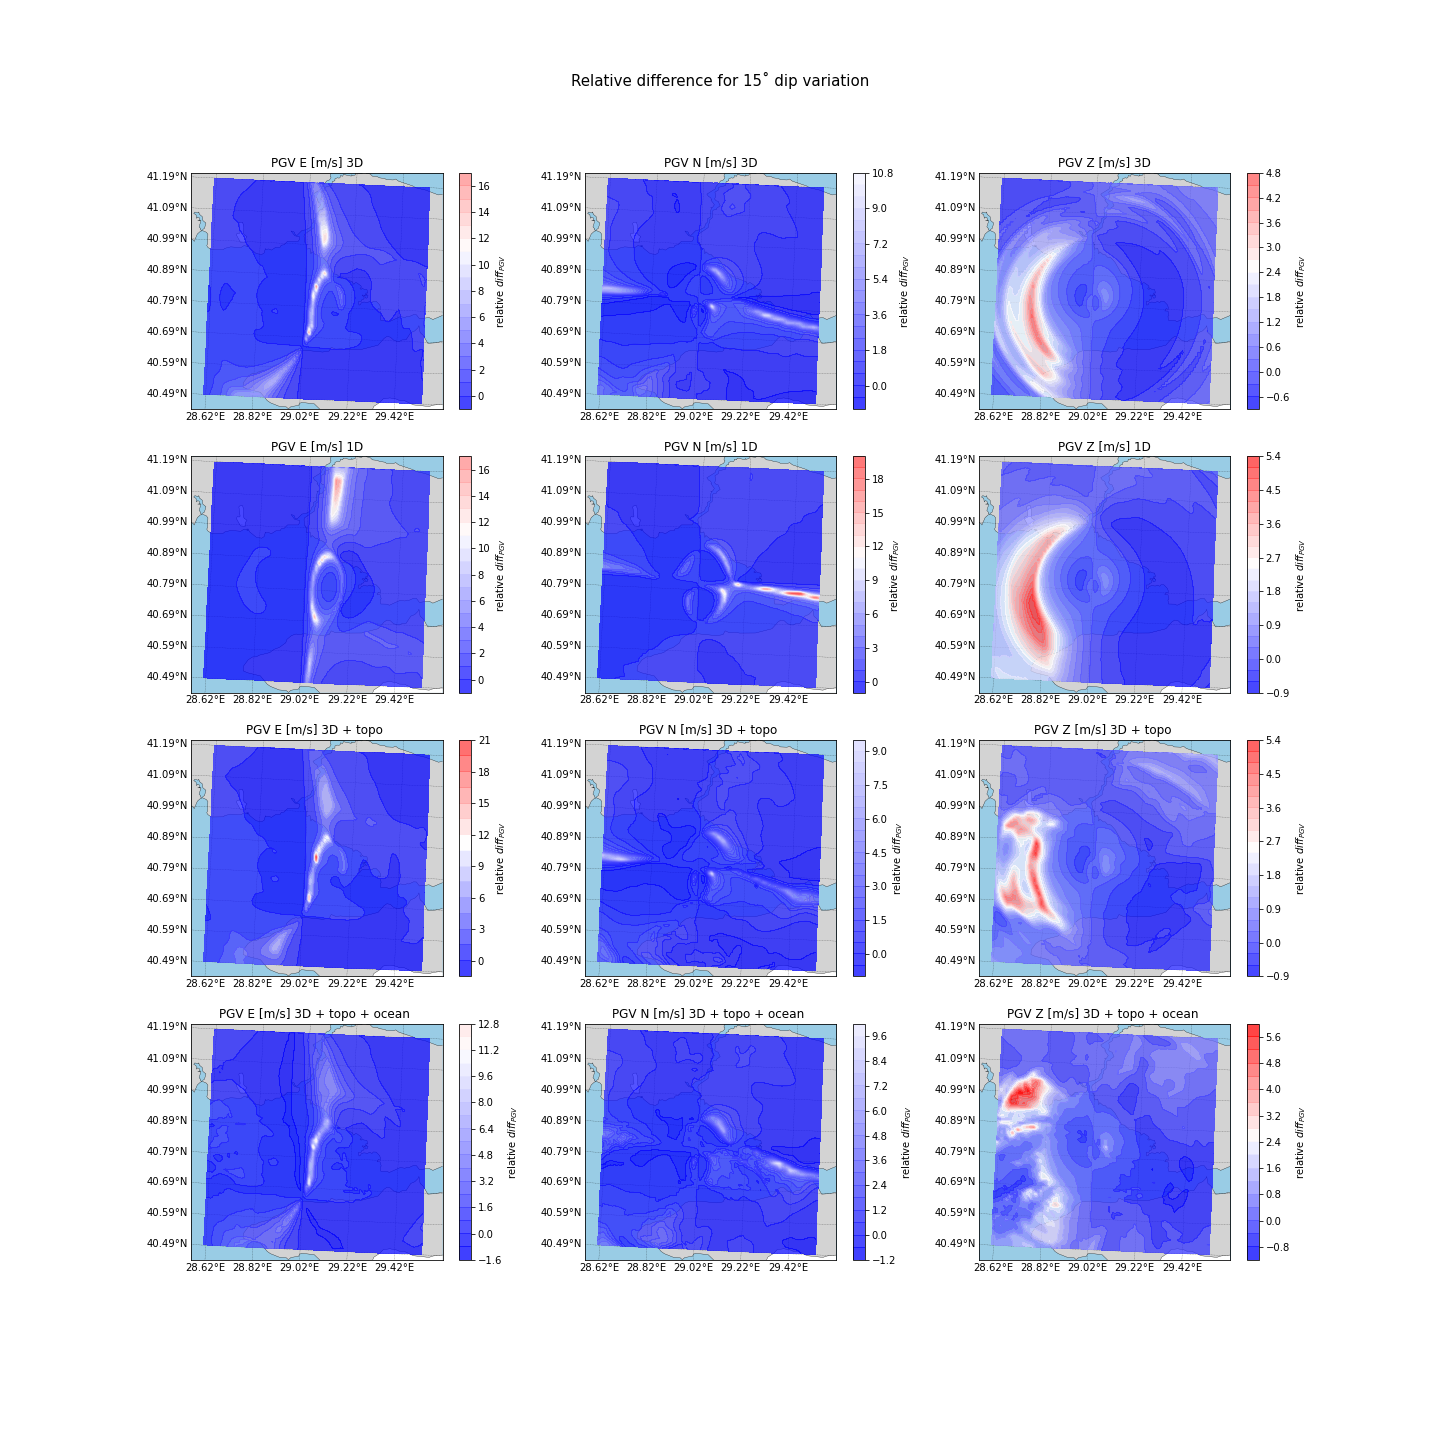
\includegraphics[width=1\linewidth]{images_results/dip_variation_epsilon12_sc4.png}
    \caption{CMT4 relative difference between a scenario with a dip variation of 11.25$\degree$ with respect to the reference scenario. Colourbar set to the total minima and maxima of the 11.25$\degree$ and 22.5$\degree$ plots for comparison.}
    \label{fig:ref_eps12-2}
\end{figure}

\FloatBarrier

\begin{figure}[!h]
    \centering
    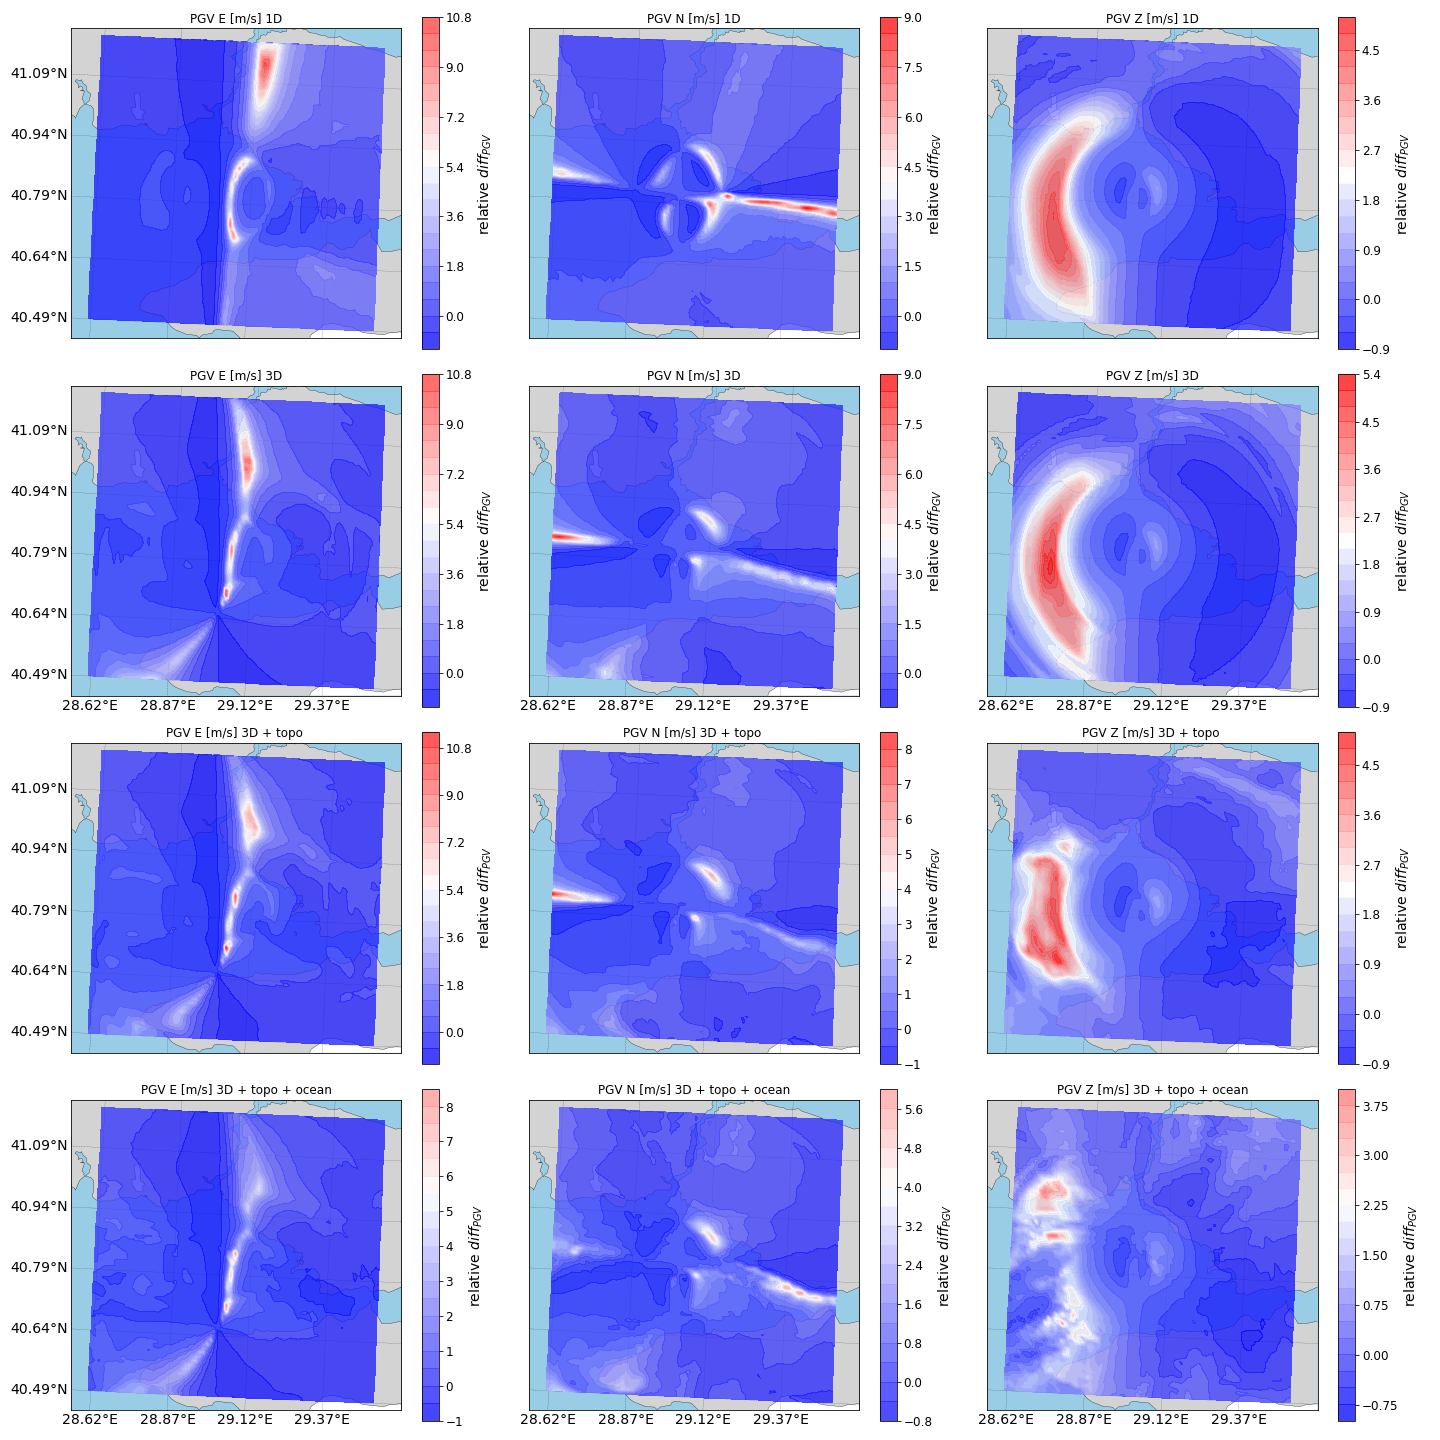
\includegraphics[width=1\linewidth]{images_results/dip_variation_epsilon25_sc4.png}
    \caption{CMT4 relative difference between a scenario with a dip variation of 22.5$\degree$ with respect to the reference scenario. Colourbar set to the total minima and maxima of the 11.25$\degree$ and 22.5$\degree$ plots for comparison.}
    \label{fig:ref_eps25-2}
\end{figure}

\FloatBarrier

\subsection{Variation rake figures CMT3 and CMT4}

\subsubsection{CMT2}

\begin{figure}
    \centering
    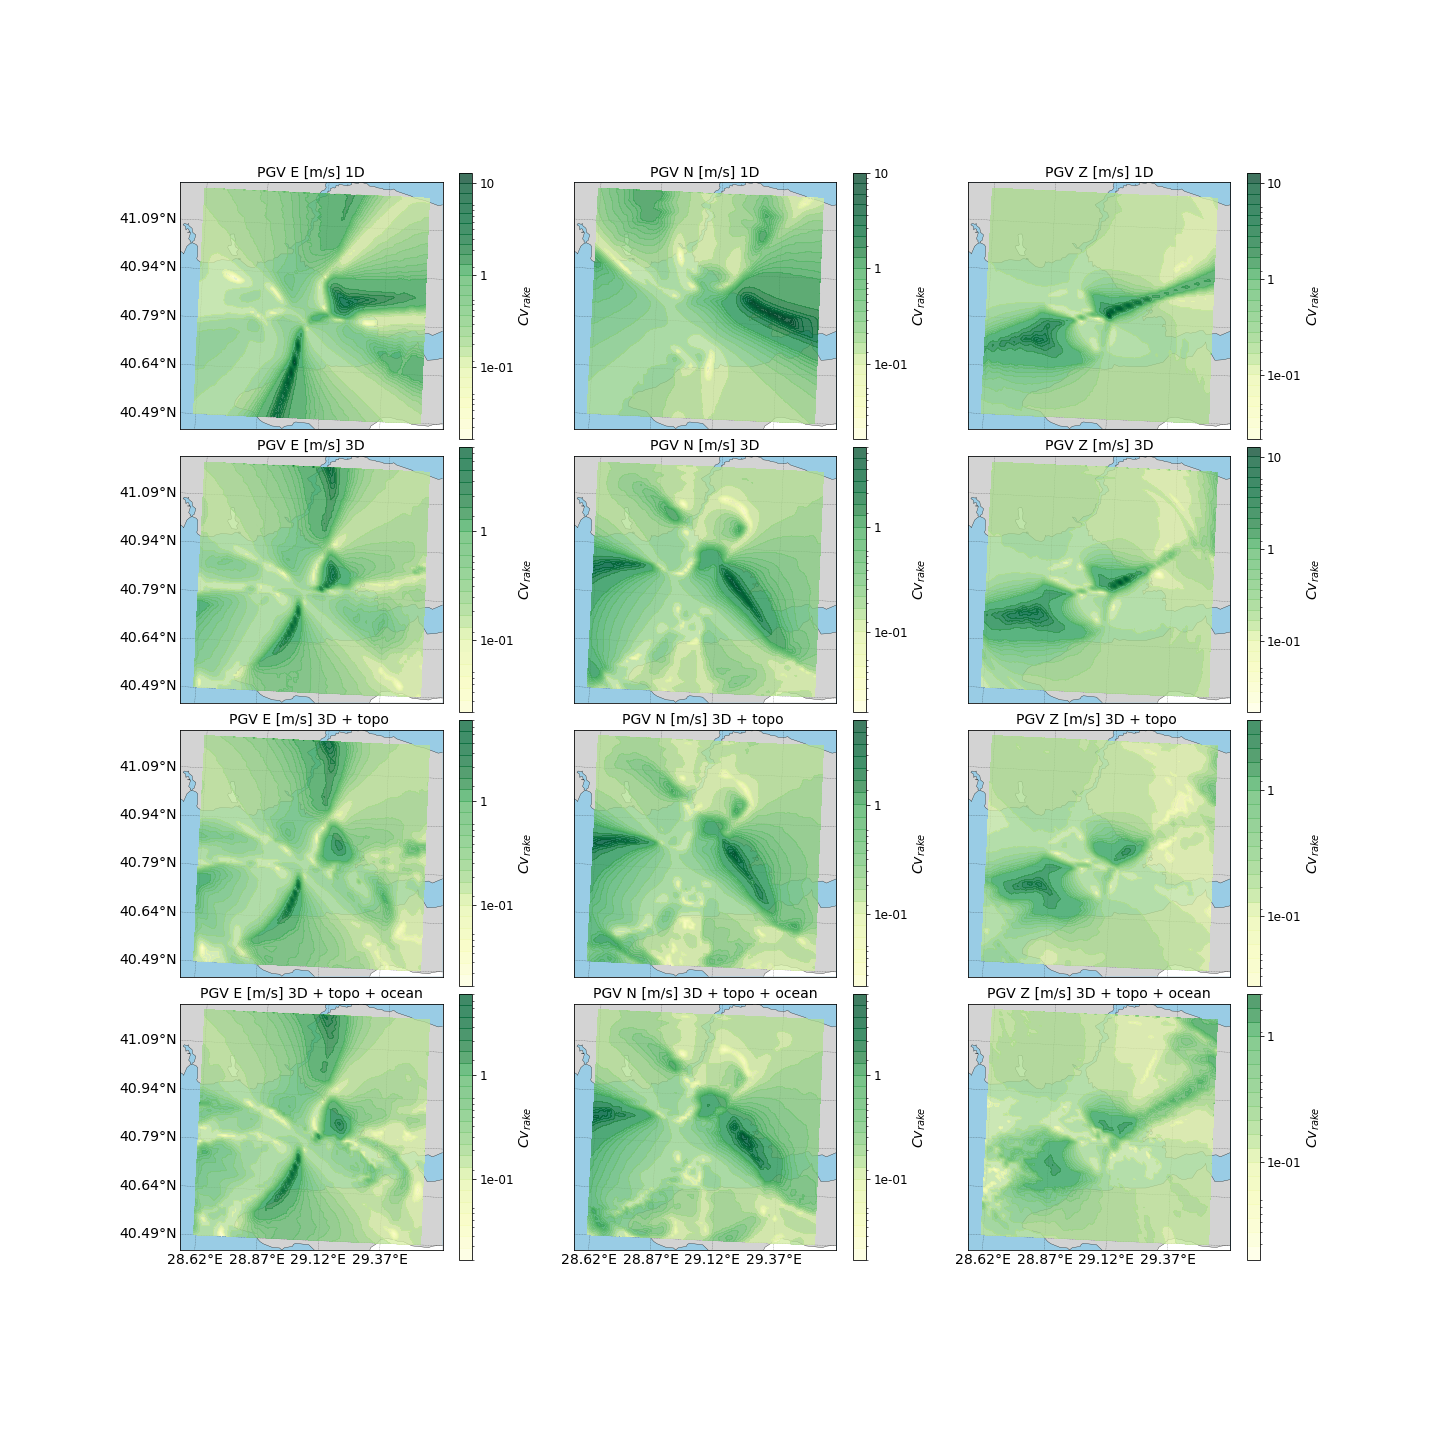
\includegraphics[width=1\linewidth,trim = 2cm 5cm 1cm 5cm, clip]{images_results/rake_variation_sigma_sc2.png}
    \caption{CMT2 coefficient of variation $Cv$ of rake variation, for each model domain in E, N and Z direction. Colourbar set to logarithmic to adequately show the large differences.}
    \label{fig:cmt2sigm}
\end{figure}


\begin{figure}[!h]
    \centering
    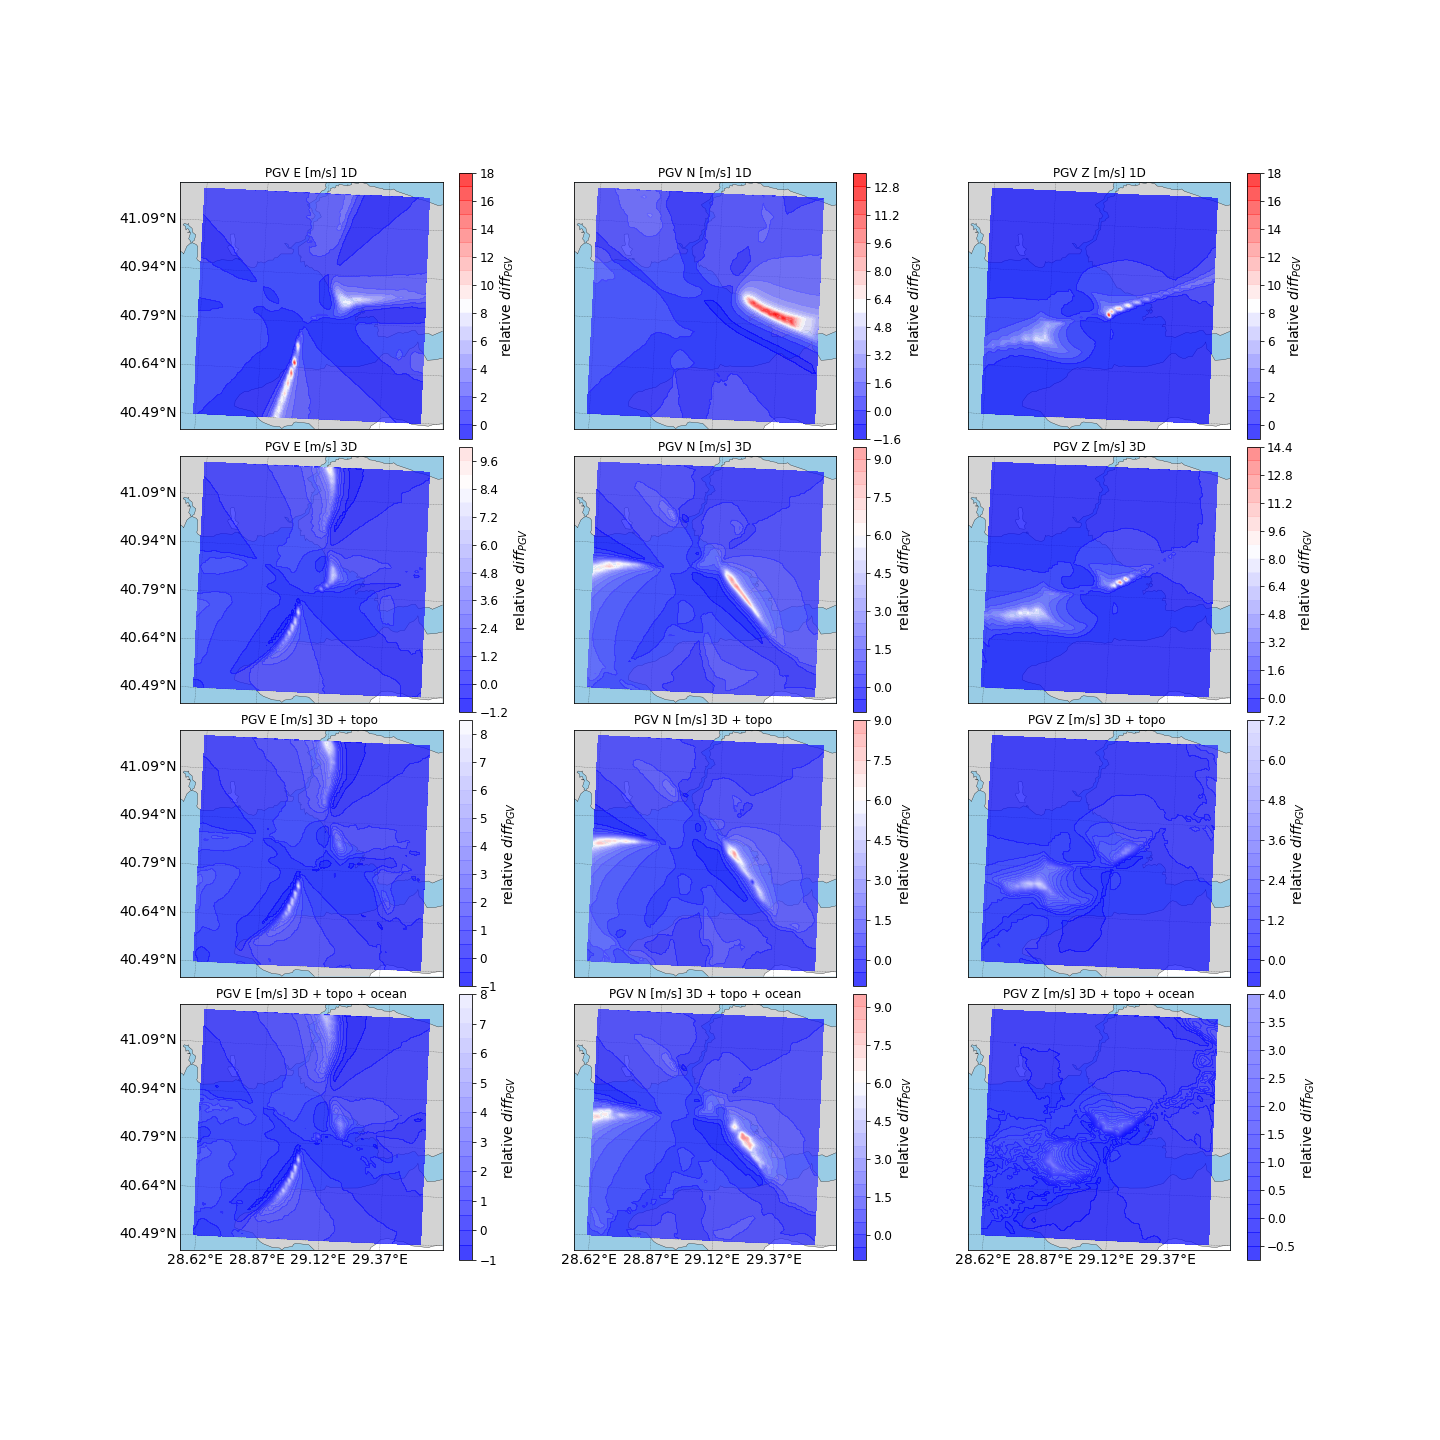
\includegraphics[width=1\linewidth,trim = 2cm 5cm 1cm 5cm, clip]{images_results/rake_variation_epsilon12_sc2.png}
    \caption{CMT3 relative difference between a scenario with a rake variation of 15$\degree$ with respect to the reference scenario. Colourbar set to the total minima and maxima of the 15$\degree$ and 30$\degree$ plots for comparison.}
    \label{fig:ref_eps12-2}
\end{figure}

\begin{figure}[!h]
    \centering
    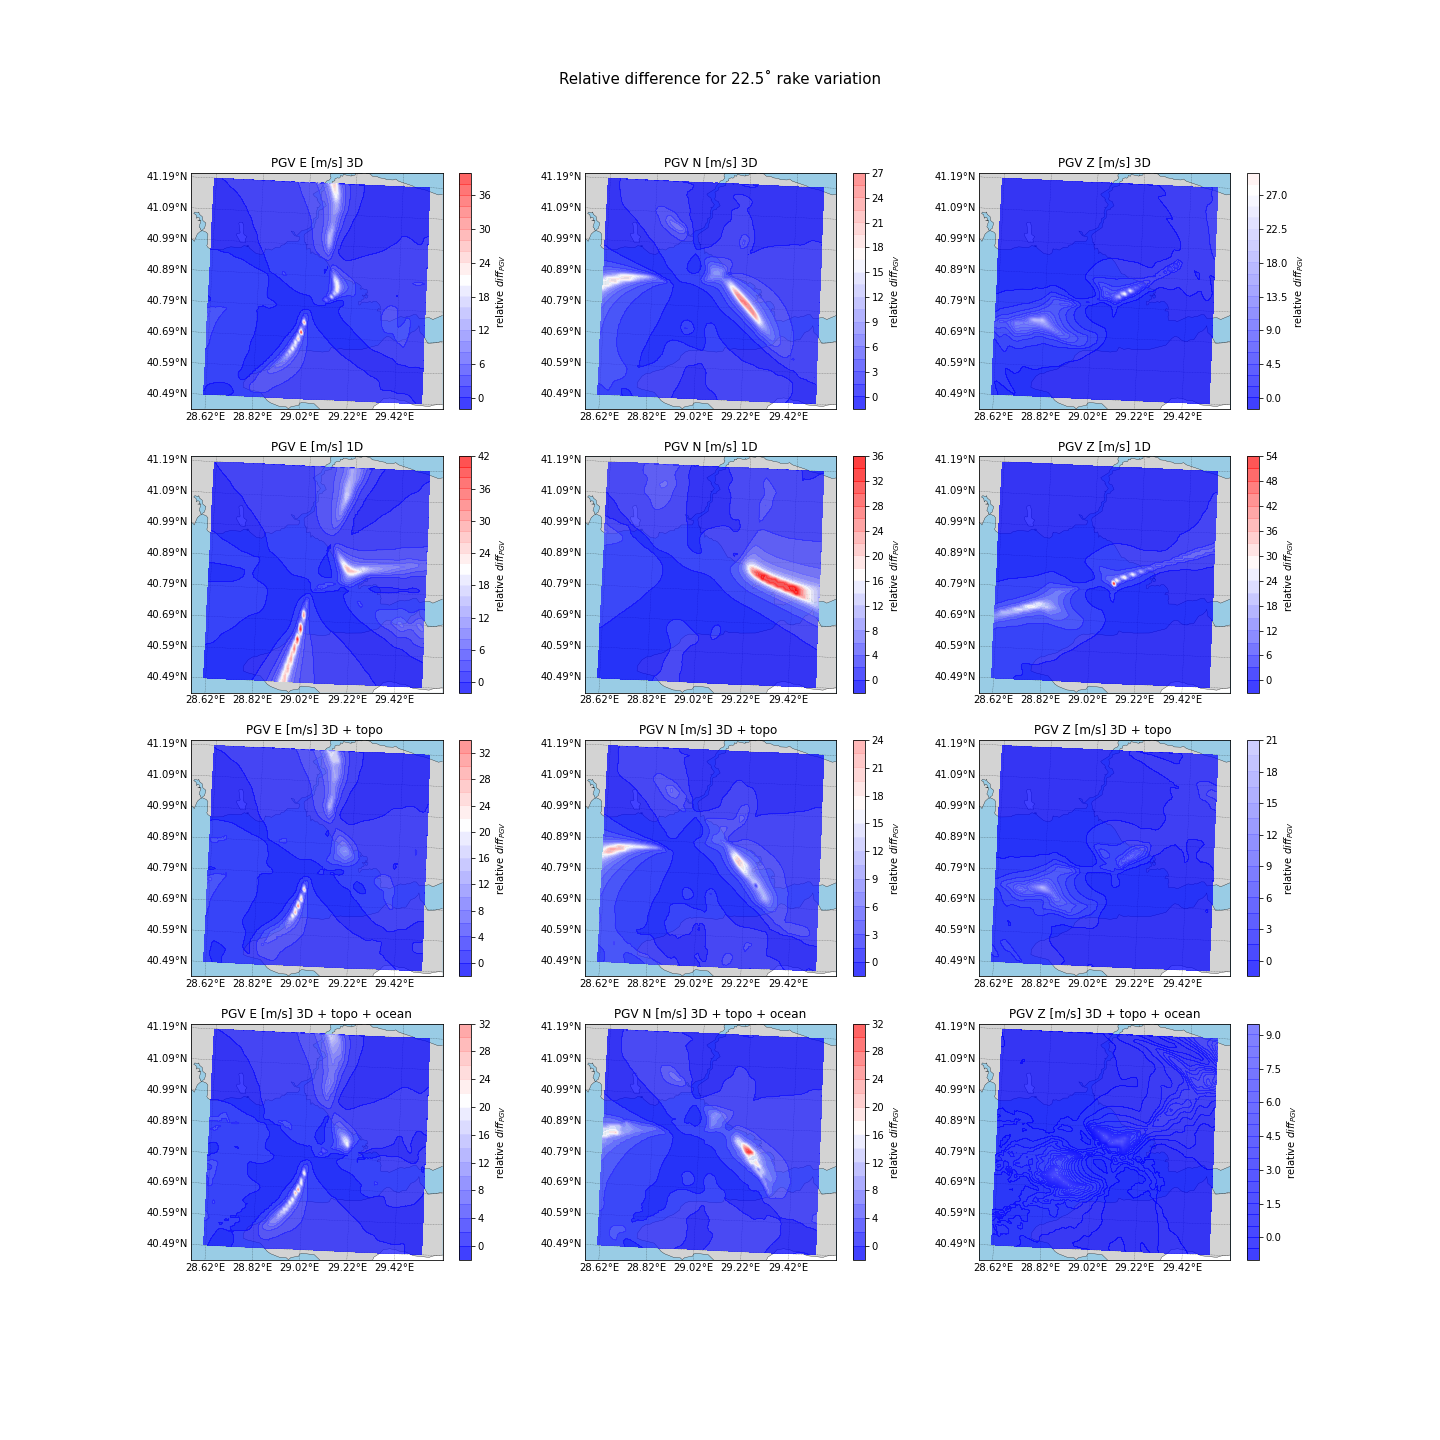
\includegraphics[width=1\linewidth,trim = 2cm 5cm 1cm 5cm, clip]{images_results/rake_variation_epsilon25_sc2.png}
    \caption{CMT3 relative difference between CMT with a rake variation of 30$\degree$ with respect to the reference scenario. Colourbar set to the total minima and maxima of the 15$\degree$ and 30$\degree$ plots for comparison.}
    \label{fig:ref_eps25-2}
\end{figure}

\subsubsection{CMT3}

\begin{figure}
    \centering
    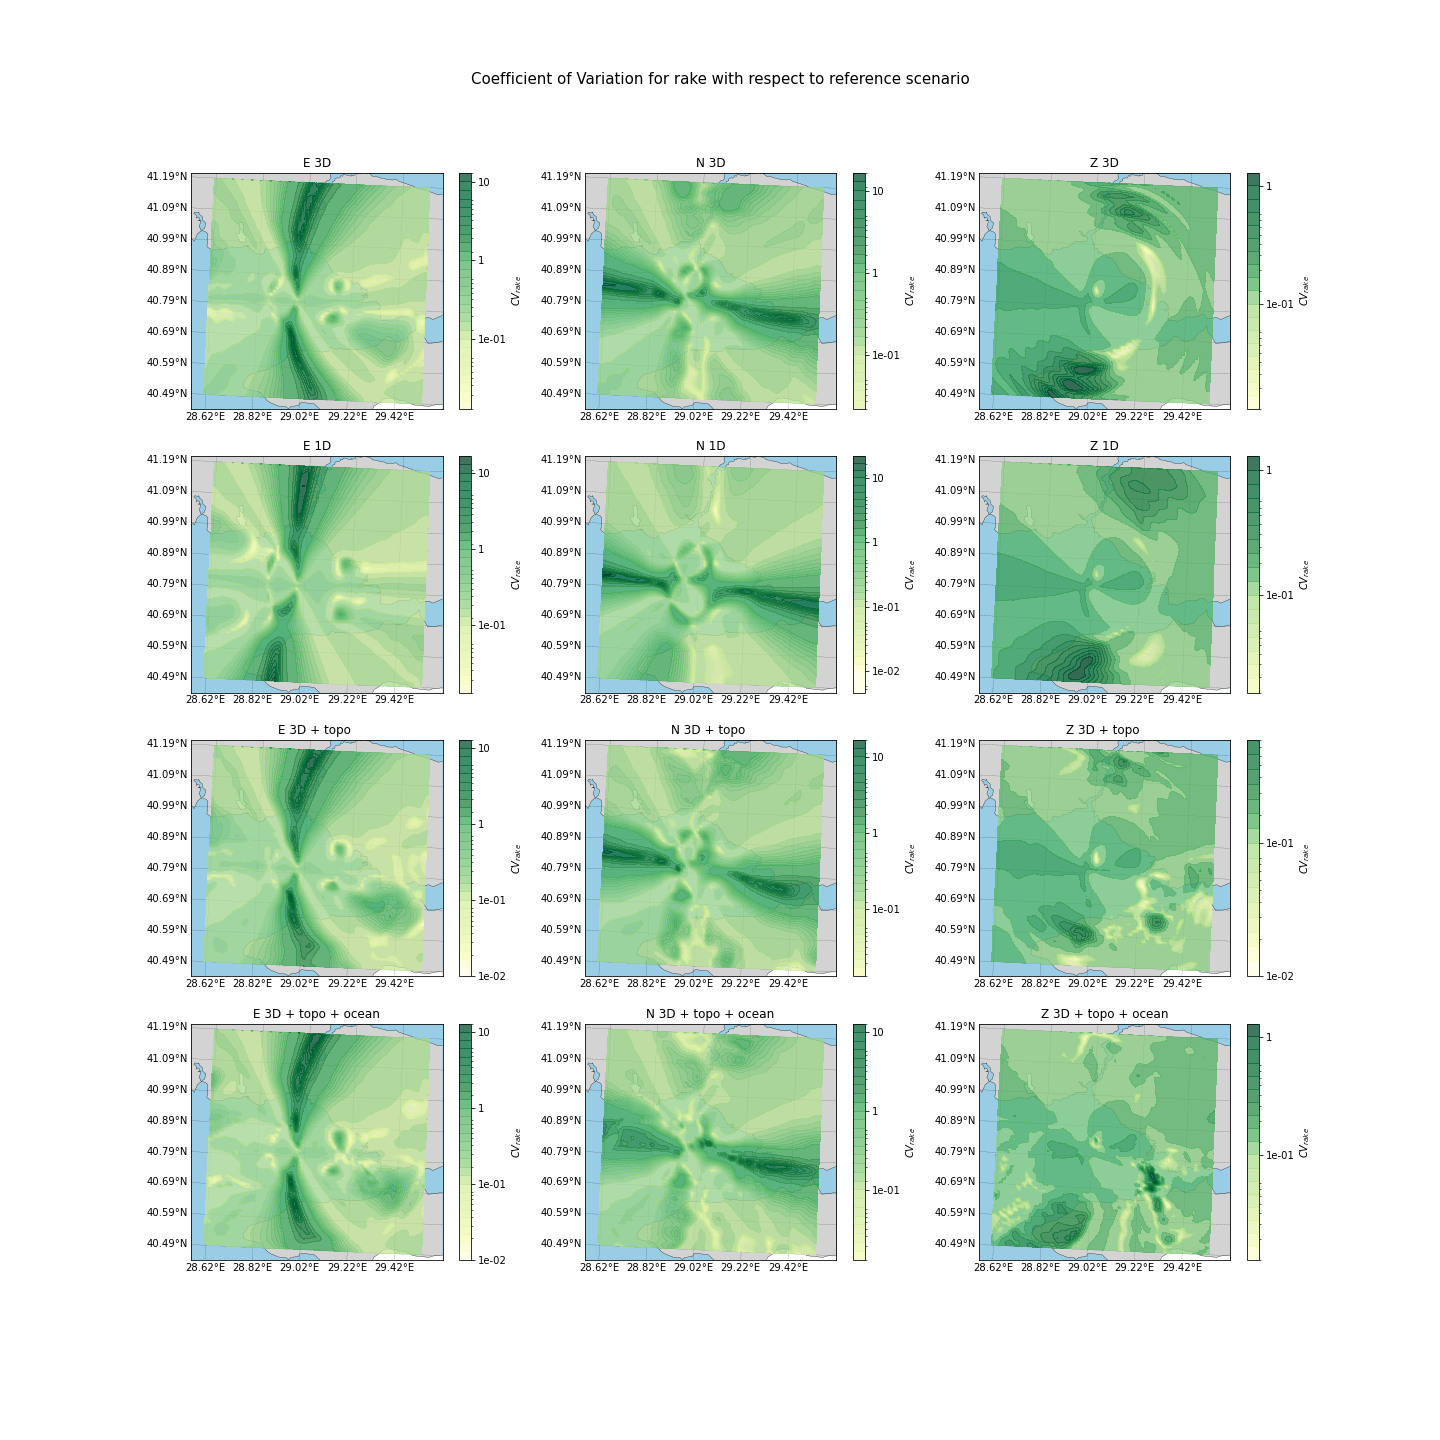
\includegraphics[width=1\linewidth,trim = 2cm 5cm 1cm 5cm, clip]{images_results/rake_variation_sigma_sc3.png}
    \caption{CMT2 coefficient of variation $Cv$ of rake variation, for each model domain in E, N and Z direction. Colourbar set to logarithmic to adequately show the large differences.}
    \label{fig:cmt2sigm}
\end{figure}


\begin{figure}[!h]
    \centering
    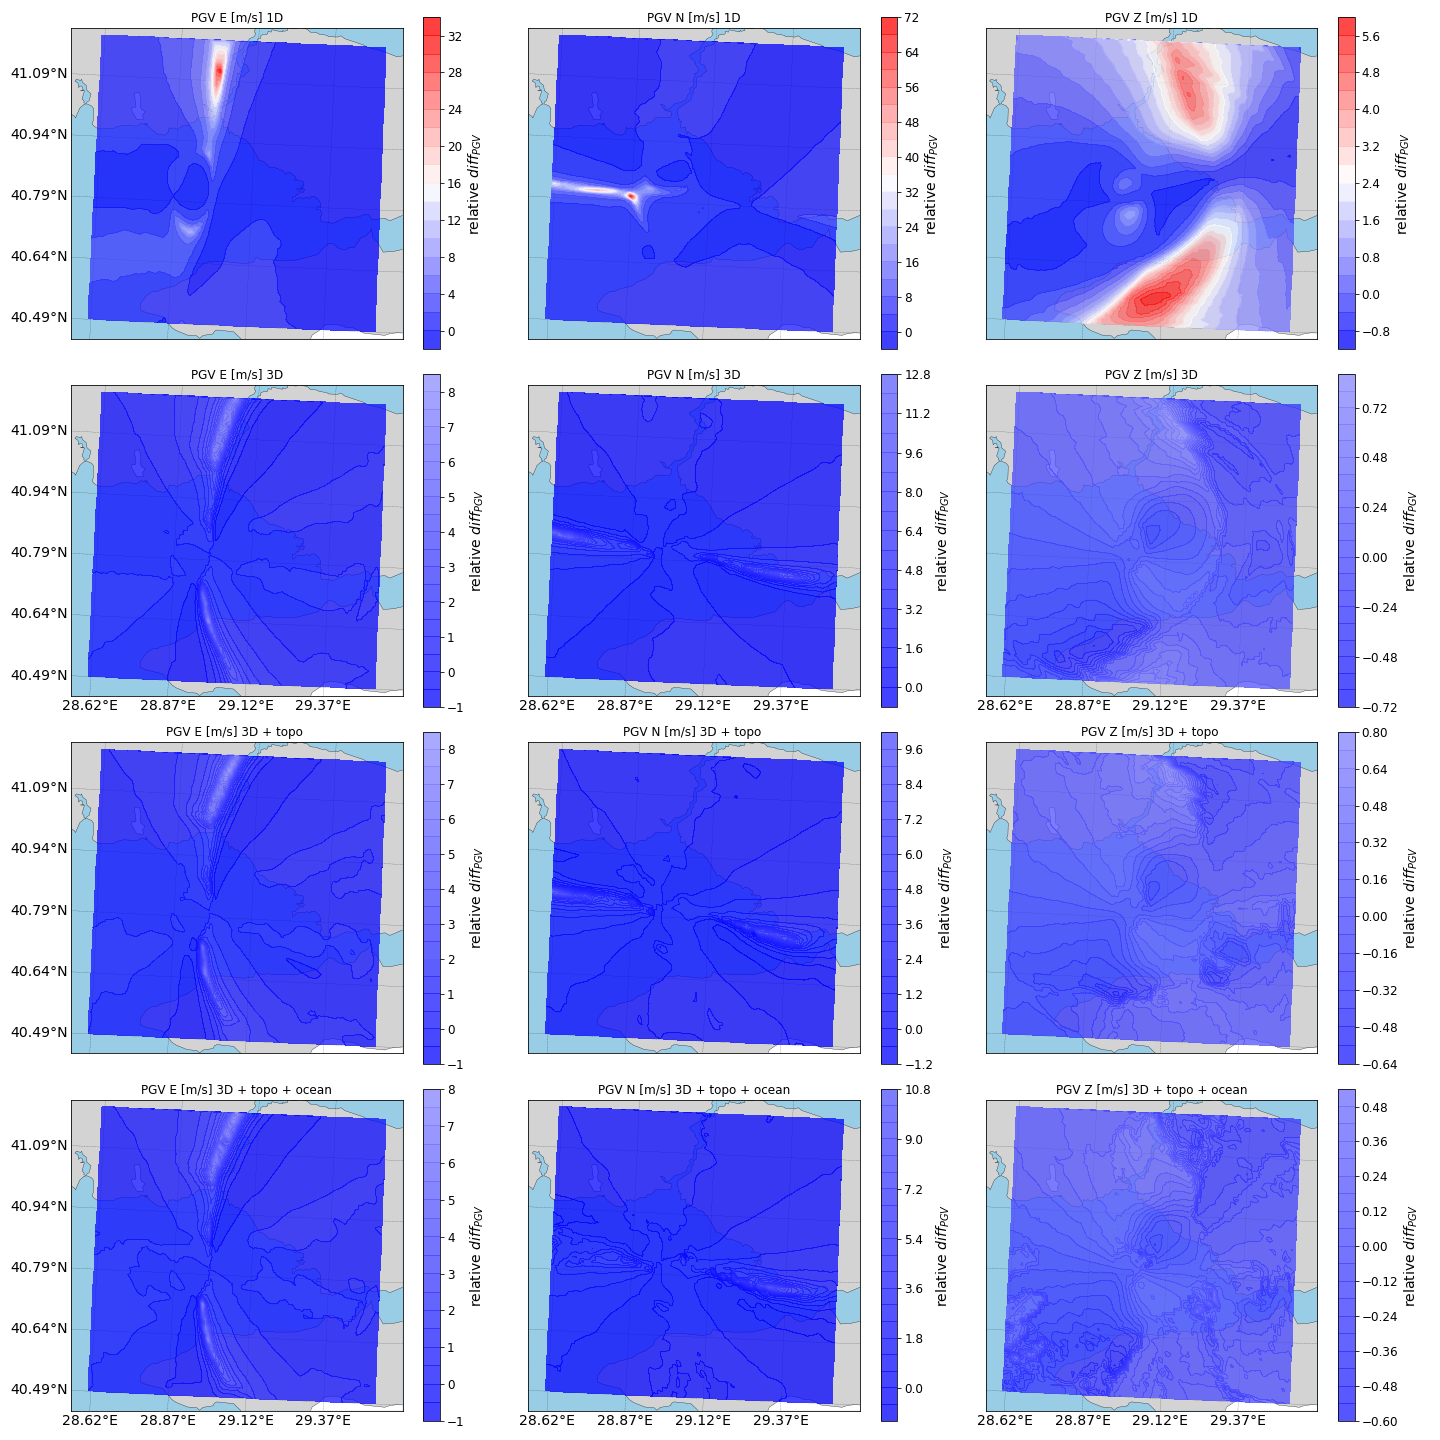
\includegraphics[width=1\linewidth,trim = 2cm 5cm 1cm 5cm, clip]{images_results/rake_variation_epsilon12_sc3.png}
    \caption{CMT3 relative difference between a scenario with a rake variation of 15$\degree$ with respect to the reference scenario. Colourbar set to the total minima and maxima of the 30$\degree$ and 30$\degree$ plots for comparison.}
    \label{fig:ref_eps12-2}
\end{figure}

\begin{figure}[!h]
    \centering
    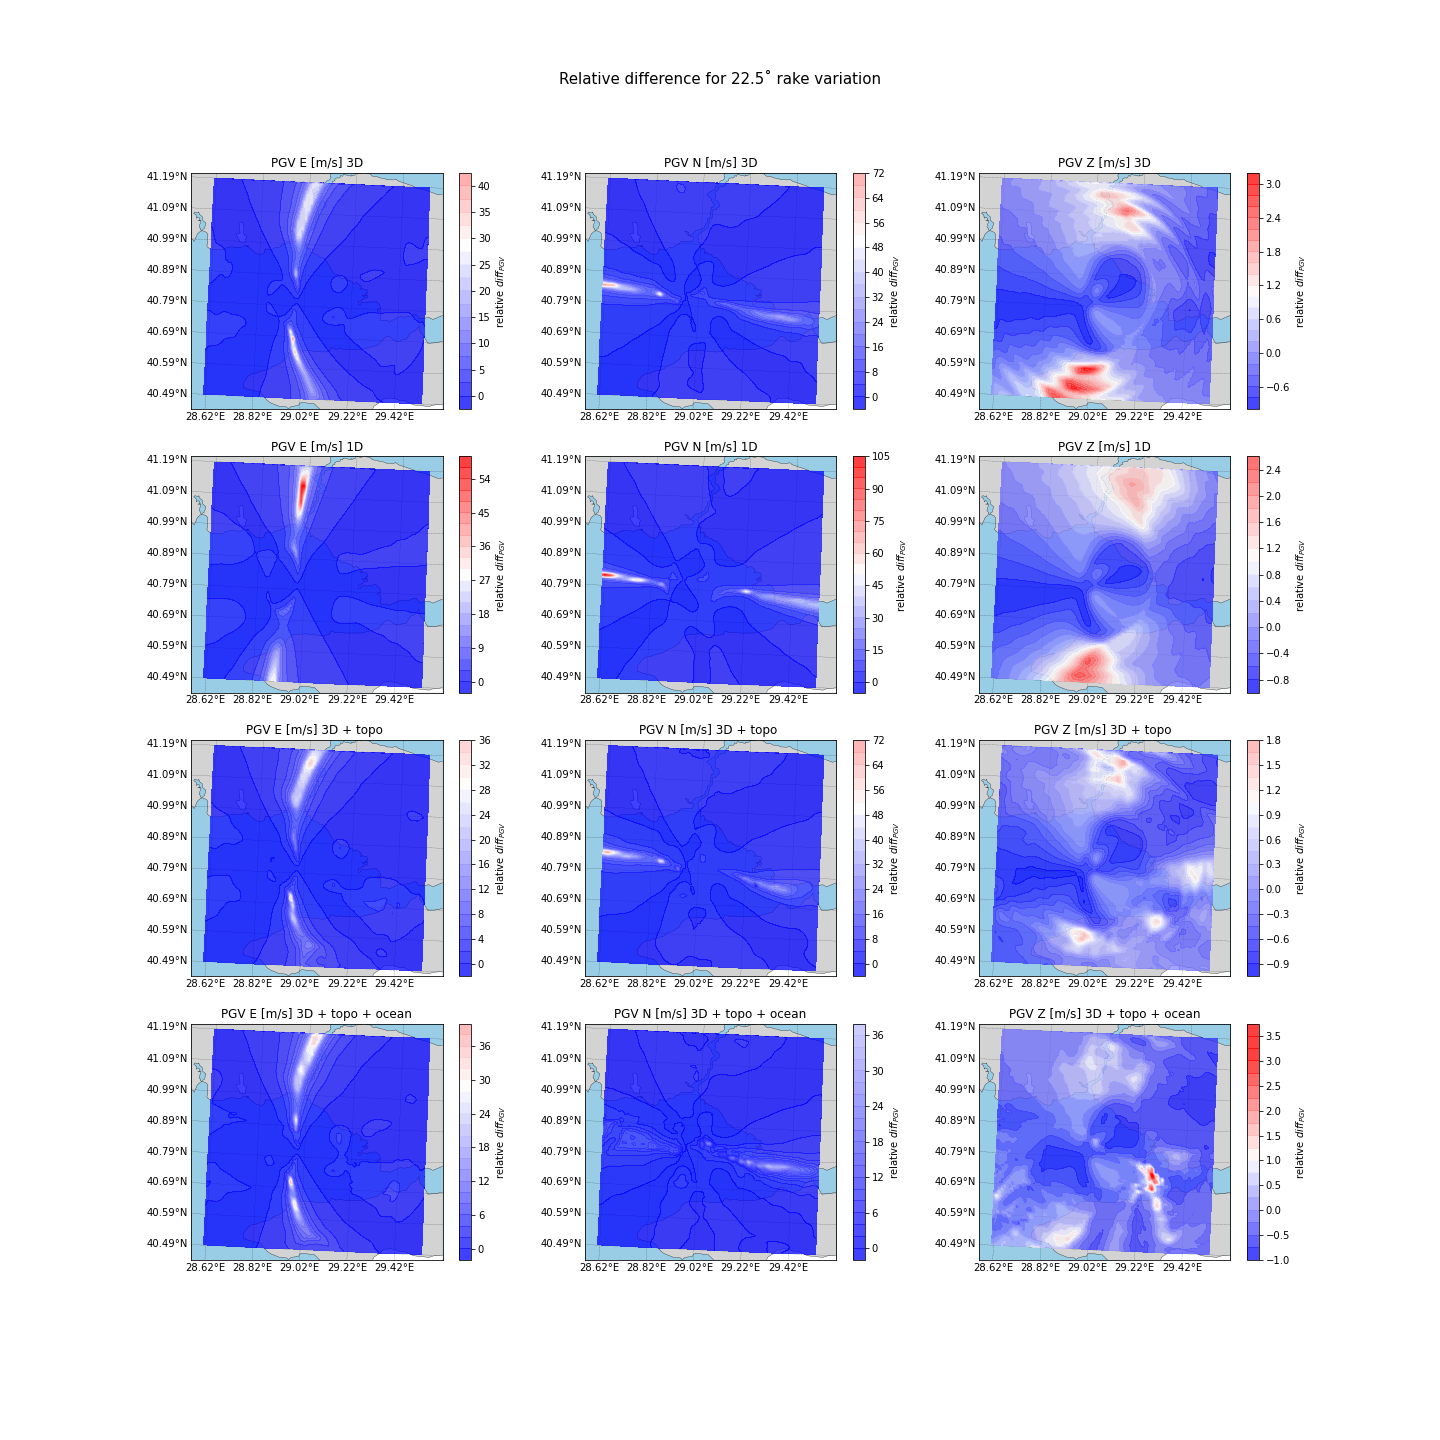
\includegraphics[width=1\linewidth,trim = 2cm 5cm 1cm 5cm, clip]{images_results/rake_variation_epsilon25_sc3.png}
    \caption{CMT3 relative difference between CMT with a rake variation of 30$\degree$ with respect to the reference scenario. Colourbar set to the total minima and maxima of the 15$\degree$ and 30$\degree$ plots for comparison.}
    \label{fig:ref_eps25-2}
\end{figure}

\FloatBarrier

\subsubsection{CMT4}

\begin{figure}[!h]
    \centering
    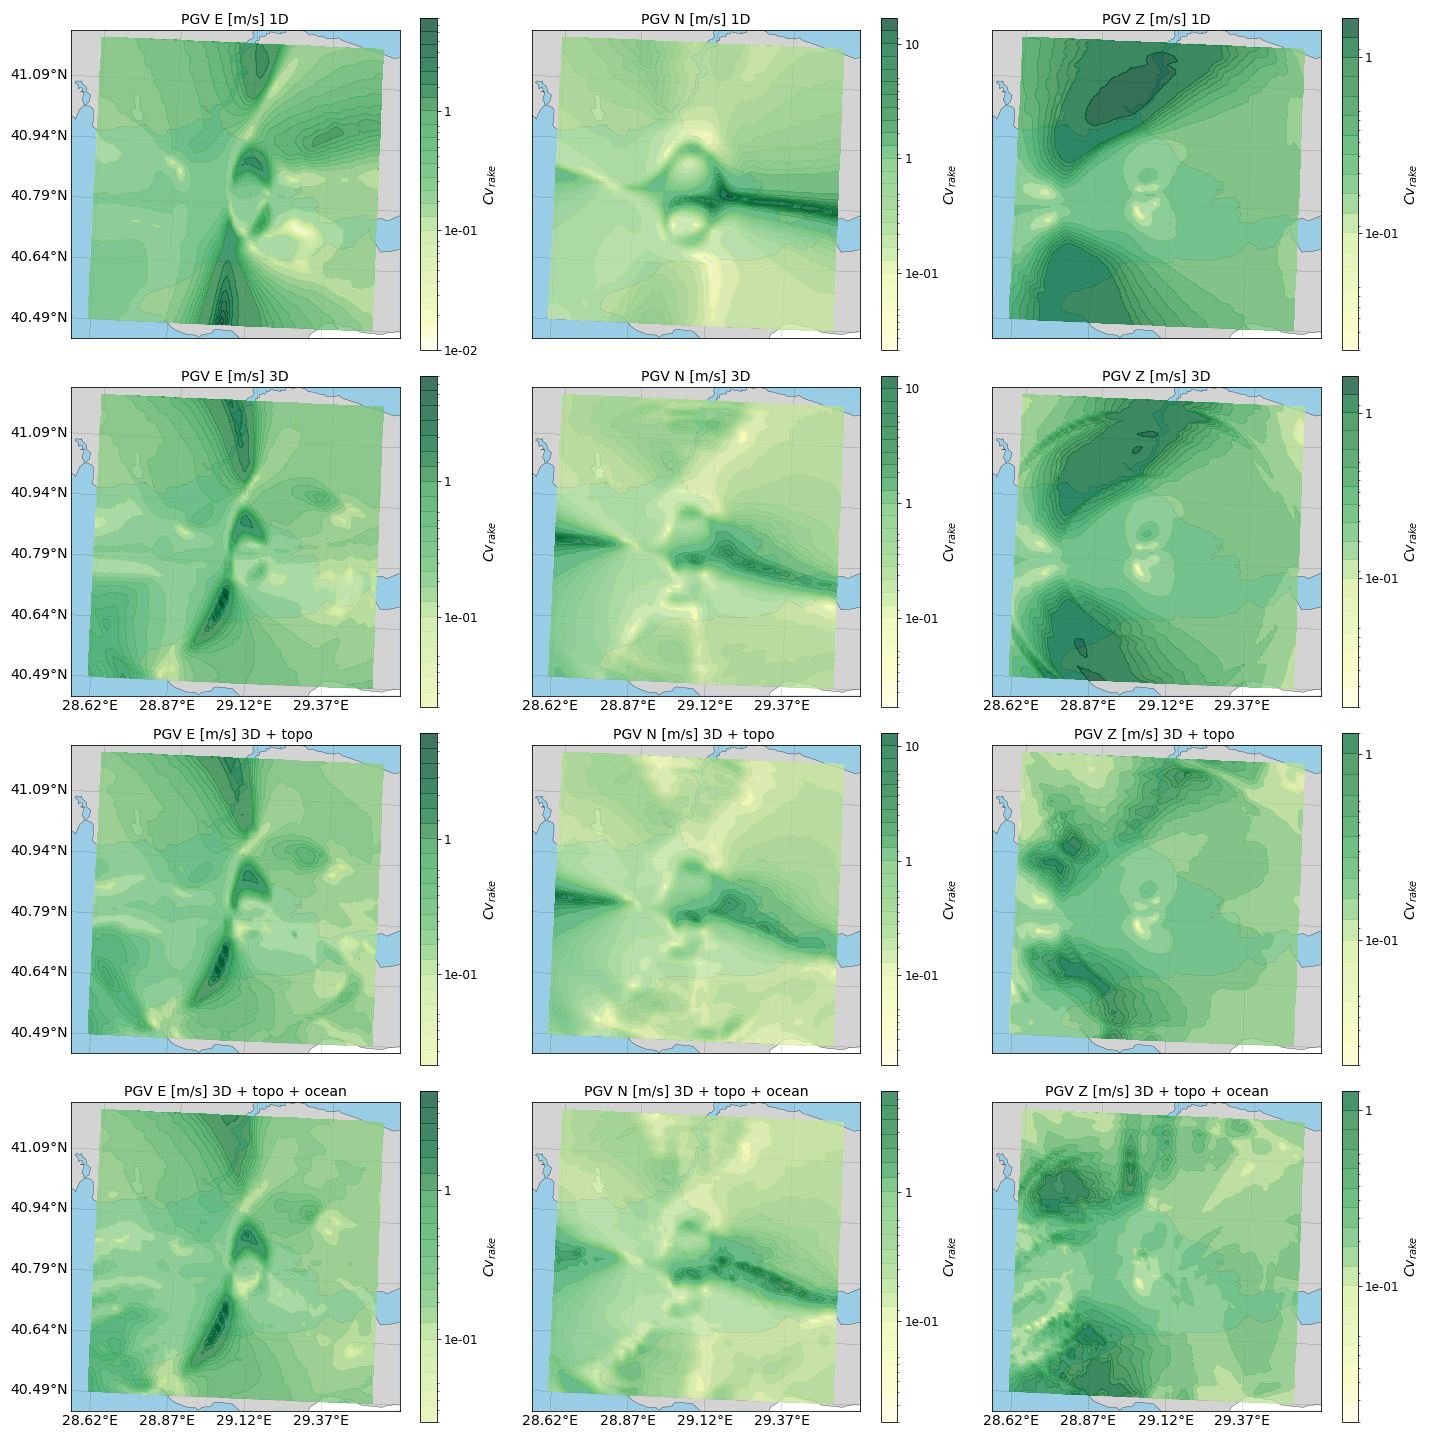
\includegraphics[width=1\linewidth]{images_results/rake_variation_sigma_sc4.png}
    \caption{CMT3 coefficient of variation $Cv$ of rake variation, for each model domain in E, N and Z direction. Colourbar set to logarithmic to adequately show the large differences.}
    \label{fig:cmt3sigm}
\end{figure}

\FloatBarrier

\begin{figure}[!h]
    \centering
    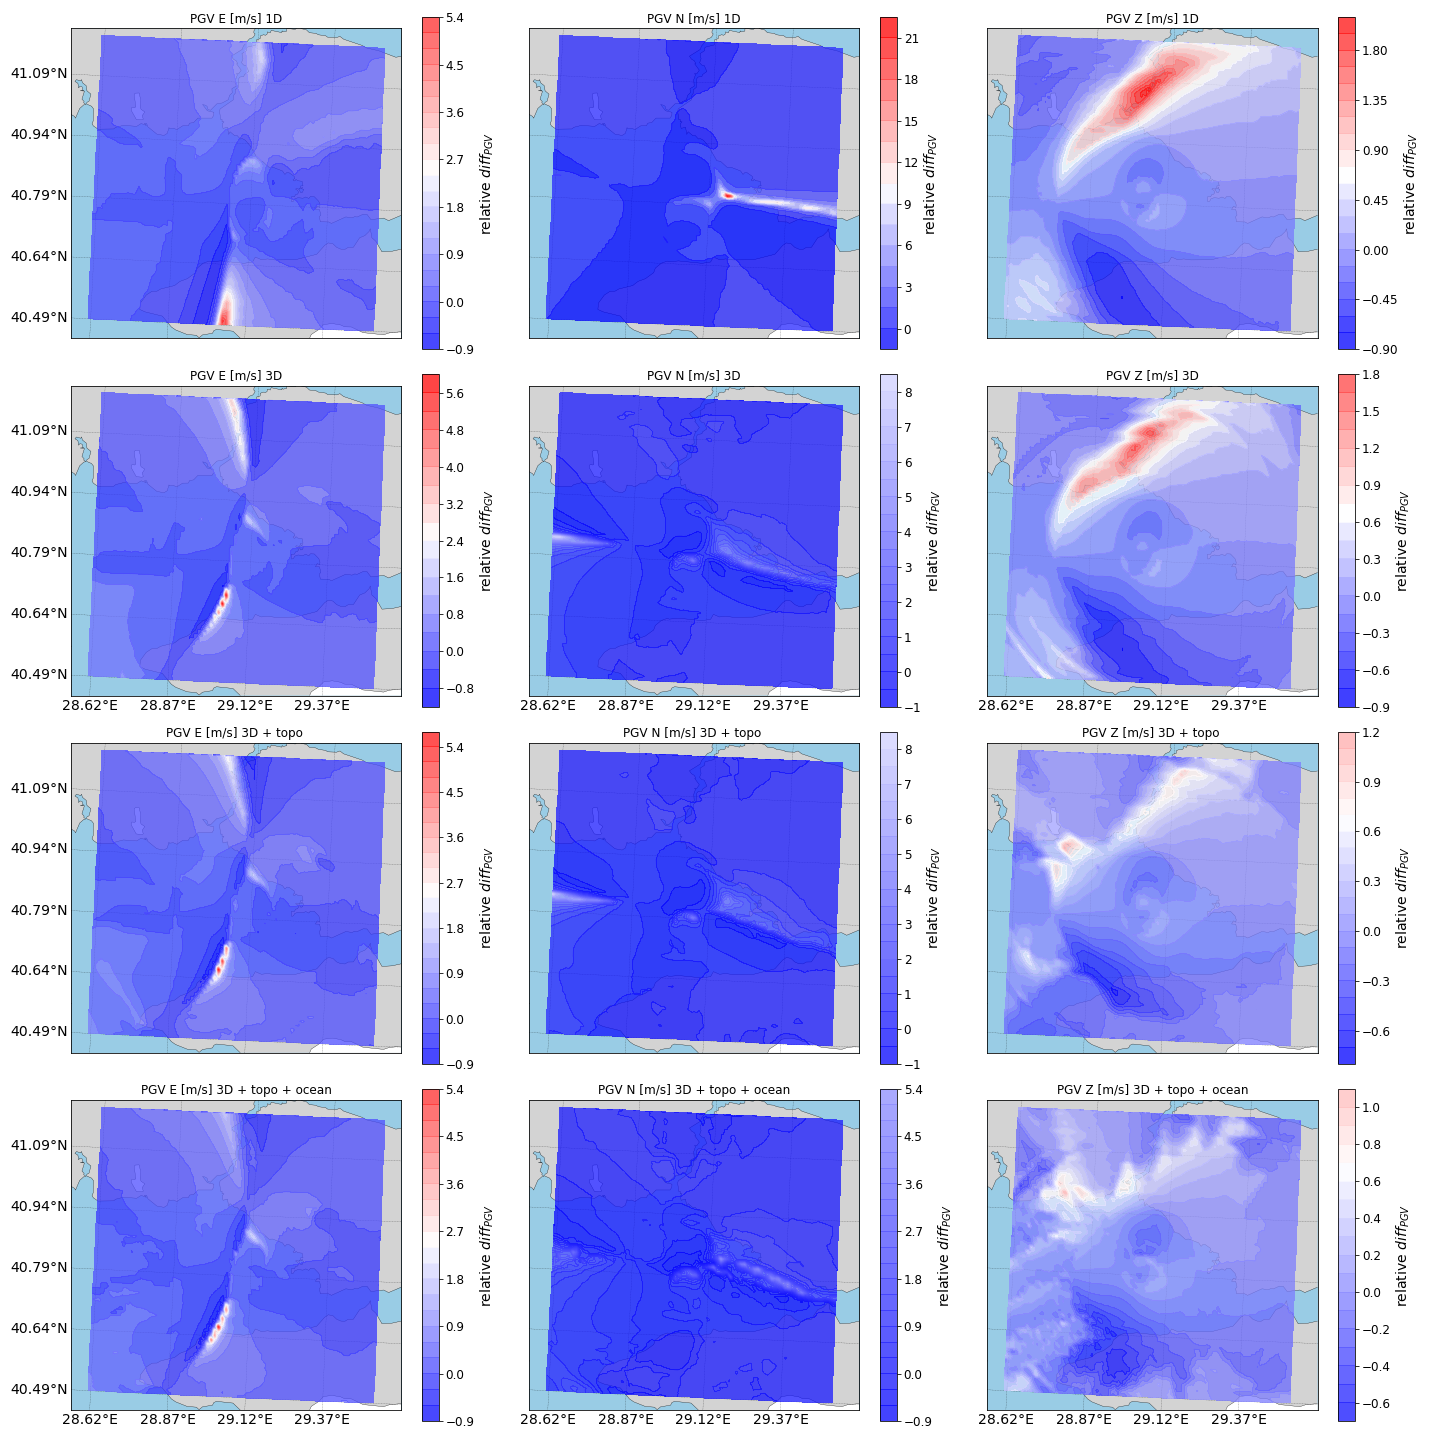
\includegraphics[width=1.2\linewidth]{images_results/rake_variation_epsilon12_sc4.png}
    \caption{CMT4 relative difference between a scenario with a strike variation of 15$\degree$ with respect to the reference scenario. Colourbar set to the total minima and maxima of the 15$\degree$ and 30$\degree$ plots for comparison.}
    \label{fig:ref_eps12-2}
\end{figure}

\FloatBarrier

\begin{figure}[!h]
    \centering
    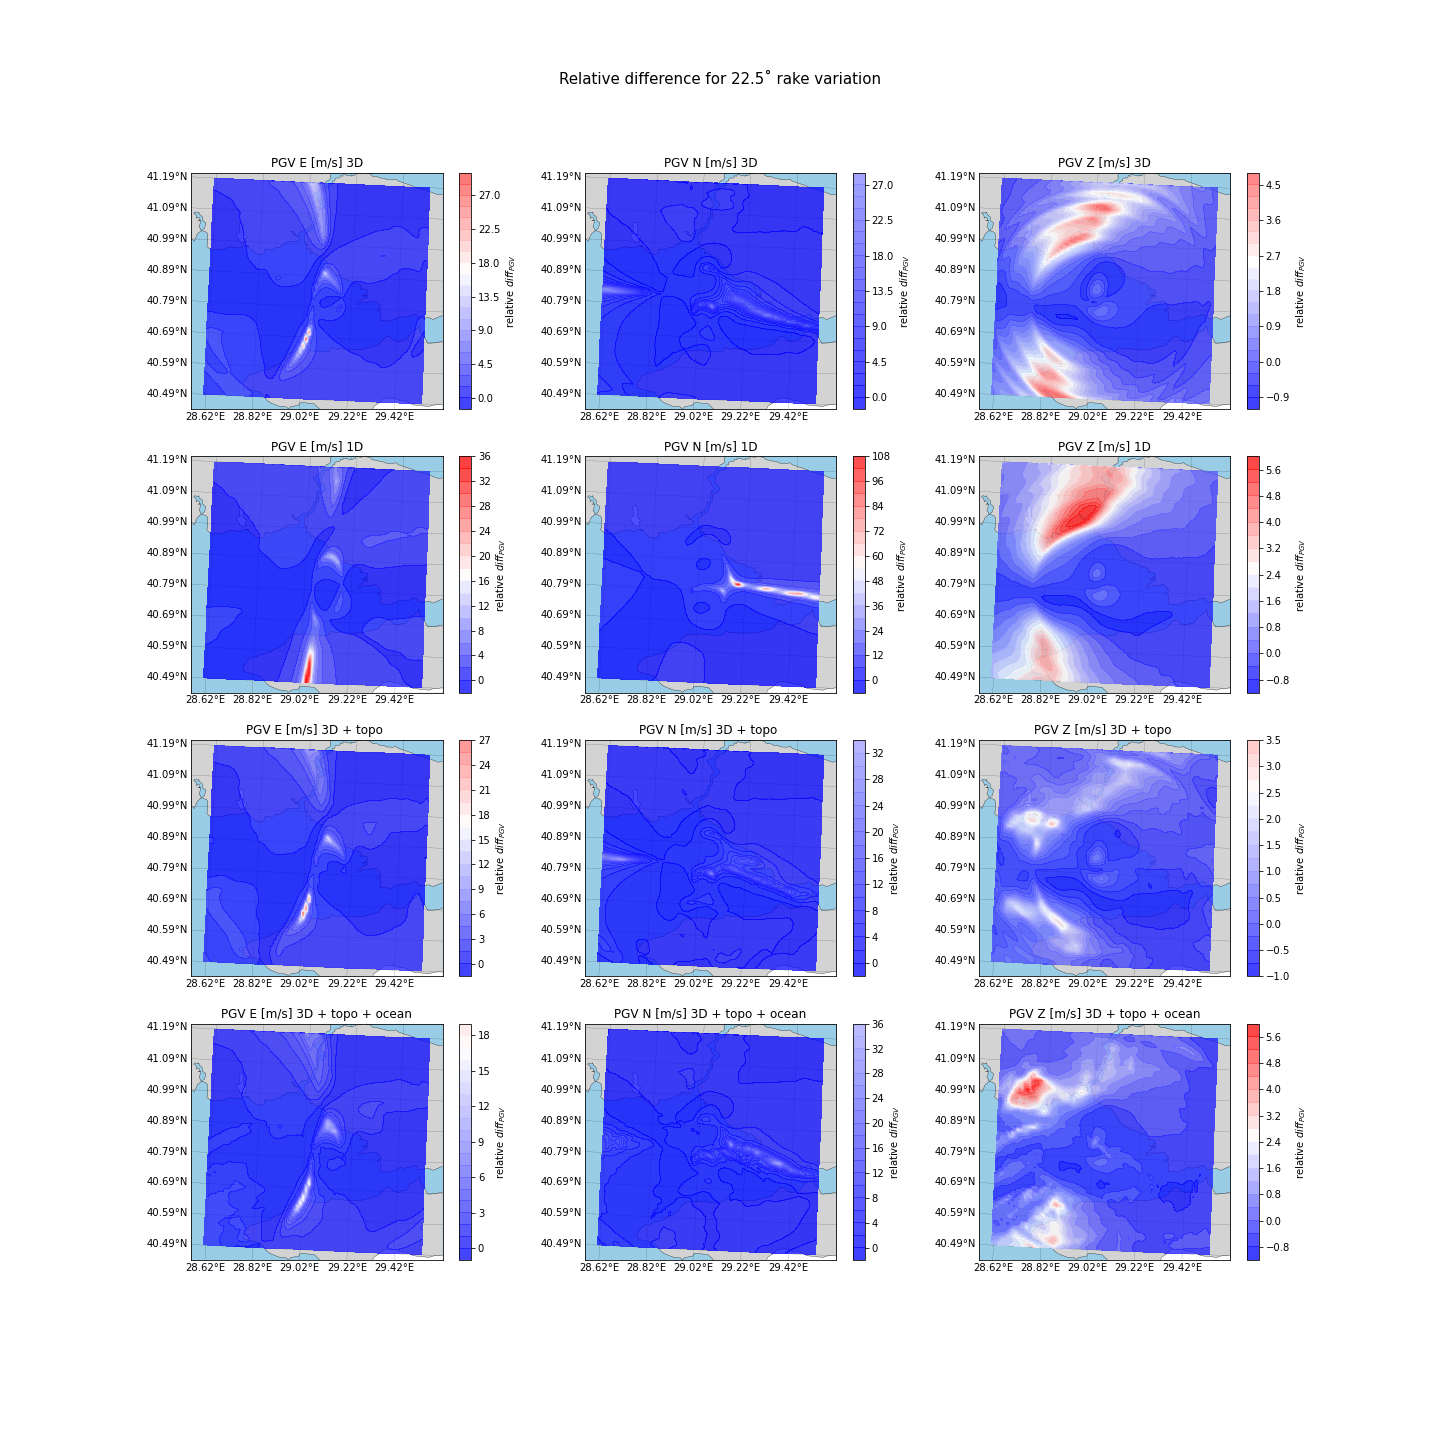
\includegraphics[width=1.2\linewidth]{images_results/rake_variation_epsilon25_sc4.png}
    \caption{CMT4 relative difference between a scenario with a strike variation of 30$\degree$ with respect to the reference scenario. Colourbar set to the total minima and maxima of the 15$\degree$ and 30$\degree$ plots for comparison.}
    \label{fig:ref_eps25-2}
\end{figure}

\FloatBarrier






\section{Other images from results}

\end{document}